\documentclass[11pt,a4paper]{article}
\newcommand{\docTitle}{Process Design Heuristics}
% preamble.tex --- shared LaTeX preamble for Choupo manuals
% Style: sober monochrome with subtle dark-blue accent for
% hyperlinks only.  Pedagogical boxes via tcolorbox.

% ---- Encoding, fonts, language --------------------------------------
\usepackage[utf8]{inputenc}
\usepackage[T1]{fontenc}
\usepackage{lmodern}
\usepackage[english]{babel}
\usepackage{microtype}
\usepackage{textcomp}

% ---- Layout ---------------------------------------------------------
\usepackage[a4paper, margin=2.4cm, headheight=15pt]{geometry}
\usepackage{fancyhdr}
\usepackage{titlesec}
\usepackage{enumitem}
\usepackage{longtable}
\usepackage{booktabs}
\usepackage{array}
\usepackage{tabularx}
\usepackage{multicol}
\usepackage{parskip}
\usepackage{needspace}
\usepackage{graphicx}

% ---- Code listings --------------------------------------------------
\usepackage{listings}
\usepackage{xcolor}

% Sober palette --- almost monochrome, one accent reserved for links
\definecolor{rulegray}{HTML}{888888}
\definecolor{lightgray}{HTML}{f4f4f4}
\definecolor{mediumgray}{HTML}{cccccc}
\definecolor{darkgray}{HTML}{555555}
\definecolor{accent}{HTML}{1c3a5a}

\lstdefinelanguage{dict}{
  morecomment=[l]{//},
  morecomment=[s]{/*}{*/},
  morestring=[b]",
}

\lstdefinelanguage{shell}{
  morecomment=[l]{\#},
}

\lstset{
  basicstyle=\ttfamily\footnotesize,
  backgroundcolor=\color{lightgray},
  frame=single,
  framerule=0.4pt,
  rulecolor=\color{mediumgray},
  numbers=none,
  showstringspaces=false,
  breaklines=true,
  breakatwhitespace=true,
  postbreak=\mbox{\textcolor{darkgray}{$\hookrightarrow$}\space},
  columns=fullflexible,
  keepspaces=true,
  xleftmargin=0.7em,
  framexleftmargin=0.7em,
  framextopmargin=0.5em,
  framexbottommargin=0.5em,
  commentstyle=\color{darkgray}\itshape,
  stringstyle=\color{black},
  language=shell,
  % No {---}/{--} -> en-dash rules: they mangle ASCII box art (the header
  % banner) and directory trees (|--...) and CLI --flags in listings.
  % Hyphens must stay literal in monospace.  Accents below ARE needed
  % (the listing font renders them via the LaTeX accent commands).
  literate={ã}{{\~a}}1 {á}{{\'a}}1 {â}{{\^a}}1
           {é}{{\'e}}1 {ê}{{\^e}}1
           {í}{{\'i}}1
           {ó}{{\'o}}1 {ô}{{\^o}}1 {õ}{{\~o}}1
           {ú}{{\'u}}1
           {ç}{{\c c}}1
           {·}{{\textperiodcentered}}1
}

% ---- PGFPlots (theory-guide figures) -------------------------------
\usepackage{pgfplots}
\pgfplotsset{compat=1.18}
\usetikzlibrary{arrows.meta, calc}

% ---- Boxes (pedagogical signposts) ----------------------------------
\usepackage[most]{tcolorbox}
\tcbuselibrary{breakable,skins}

\newtcolorbox{keyidea}{
  breakable,
  colback=lightgray,
  colframe=black,
  boxrule=0.4pt,
  arc=1pt,
  left=10pt,right=10pt,top=6pt,bottom=6pt,
  before upper={\noindent\textbf{\sffamily Key idea.}\quad},
}

\newtcolorbox{pitfall}{
  breakable,
  colback=white,
  colframe=darkgray,
  boxrule=0.4pt,
  arc=1pt,
  left=10pt,right=10pt,top=6pt,bottom=6pt,
  before upper={\noindent\textbf{\sffamily Common pitfall.}\quad},
}

\newtcolorbox{tryit}{
  breakable,
  colback=lightgray,
  colframe=darkgray,
  boxrule=0.4pt,
  arc=1pt,
  left=10pt,right=10pt,top=6pt,bottom=6pt,
  before upper={\noindent\textbf{\sffamily Try it now.}\quad},
}

\newtcolorbox{whatyoulllearn}{
  breakable,
  colback=white,
  colframe=black,
  boxrule=0pt,
  leftrule=2pt,
  arc=0pt,
  outer arc=0pt,
  left=10pt,right=4pt,top=2pt,bottom=2pt,
  before upper={\noindent\textit{\sffamily\small What you'll learn.}\quad},
}

% Worked example --- the pedagogical workhorse of the theory manual.
\newcounter{theoryexample}[section]
\renewcommand{\thetheoryexample}{\thesection.\arabic{theoryexample}}
\newtcolorbox{example}[1][]{
  breakable,
  colback=lightgray,
  colframe=black,
  boxrule=0.4pt,
  arc=1pt,
  left=10pt,right=10pt,top=6pt,bottom=6pt,
  title={\textbf{\sffamily Worked example~\thetheoryexample.}\enspace #1},
  fonttitle=\sffamily,
  coltitle=black,
  attach title to upper,
  before title={\refstepcounter{theoryexample}},
}

% Intuition --- a one-paragraph sense-making aside, marked by a left rule.
\newtcolorbox{intuition}{
  breakable,
  colback=white,
  colframe=black,
  boxrule=0pt,
  leftrule=2pt,
  arc=0pt,
  outer arc=0pt,
  left=10pt,right=4pt,top=2pt,bottom=2pt,
  before upper={\noindent\textit{\sffamily\small Intuition.}\quad},
}

% Link-back to a tutorial --- visual cue that this maps to a runnable case.
\newtcolorbox{tutoriallink}{
  breakable,
  colback=white,
  colframe=darkgray,
  boxrule=0pt,
  leftrule=2pt,
  arc=0pt,
  outer arc=0pt,
  left=10pt,right=4pt,top=2pt,bottom=2pt,
  before upper={\noindent\textbf{\sffamily\small Runnable case.}\quad},
}

% ---- Headers/footers ------------------------------------------------
\pagestyle{fancy}
\fancyhf{}
\renewcommand{\sectionmark}[1]{\markboth{\thesection\quad #1}{}}
\fancyhead[L]{\small\sffamily\nouppercase{\leftmark}}
\fancyhead[R]{\small\sffamily\thepage}
\fancyfoot[C]{\small\sffamily Choupo-2607}
\renewcommand{\headrulewidth}{0.3pt}
\renewcommand{\footrulewidth}{0pt}

\let\choupoSection\section
\renewcommand{\section}{\clearpage\choupoSection}

% ---- Section titles -------------------------------------------------
\titleformat{\section}
  {\Large\bfseries\sffamily}{\thesection}{0.8em}{}[\vspace{-0.4em}\rule{\linewidth}{0.3pt}]
\titleformat{\subsection}
  {\large\bfseries\sffamily}{\thesubsection}{0.8em}{}
\titleformat{\subsubsection}
  {\normalsize\bfseries\sffamily}{\thesubsubsection}{0.8em}{}

\titlespacing*{\section}{0pt}{2.0ex plus 1ex minus.2ex}{1.0ex plus.2ex}
\titlespacing*{\subsection}{0pt}{1.6ex plus 1ex minus.2ex}{0.8ex plus.2ex}

% ---- Hyperref last --------------------------------------------------
\usepackage[colorlinks=true,
            linkcolor=accent,
            citecolor=accent,
            urlcolor=accent,
            bookmarksnumbered=true,
            destlabel=true,        % \label{ch:cstr} -> PDF named destination "ch:cstr"
            pdfborder={0 0 0}]{hyperref}

% ---- Shortcuts ------------------------------------------------------
\newcommand{\code}[1]{\texttt{#1}}
\newcommand{\file}[1]{\texttt{#1}}
\newcommand{\dict}[1]{\texttt{#1}}
\newcommand{\cpp}{C\texttt{++}}

% Manual authorship is selected by each guide before loading this preamble.
% Properties/Theory: Vitor, Pedro, Miguel. All other guides: Vitor alone.
\newcommand{\manualauthors}{%
  \ifdefined\propertyTheoryAuthors
    V\'{\i}tor Geraldes, Pedro Mendes, and Miguel Rodrigues%
  \else
    V\'{\i}tor Geraldes%
  \fi}

% OpenFOAM-style manual front matter: title page, then a copyright/licence
% notice page.  No source-code banner belongs on manual covers.
\newcommand{\manualfrontmatter}[2]{%
  \begin{titlepage}
  \thispagestyle{empty}
  \vspace*{2.0cm}
  \begin{center}
  
\includegraphics[height=4.0cm]{../gui/public/logo2-mark.png}\\[0.8cm]
  {\Huge\bfseries\sffamily Choupo}\\[0.35cm]
  {\Large\sffamily The Open Source Chemical Process Simulator}\\[1.3cm]
  {\Huge\bfseries\sffamily #1}\\[0.7cm]
  {Version 2607}\\[0.1cm]
  {30 June 2026}
  \end{center}
  \end{titlepage}

  \clearpage
  \thispagestyle{empty}
  \vspace*{1.2cm}
  \noindent Copyright \textcopyright{} 2026 \manualauthors.\\[0.3cm]
  \noindent Authors: \manualauthors.\\[0.3cm]
  \noindent This work is licensed under a Creative Commons
  Attribution-ShareAlike 4.0 International License.\\[0.3cm]
  \noindent Code examples, Choupo case files, and other machine-readable
  examples are licensed under GPL-3.0-or-later.\\[0.3cm]
  \noindent Typeset in \LaTeX.

  \vspace{1.0cm}
  \noindent\rule{\linewidth}{0.3pt}
  \noindent\footnotesize\textit{Acknowledgment.}\quad Choupo was conceived and
  architected by V\'{\i}tor Geraldes. Substantial parts of the initial
  implementation, documentation, and tutorial corpus were produced with
  assistance from Anthropic Claude Code using Claude Opus/Fable models. This
  guide is published under human curation, review, and editorial responsibility
  by \manualauthors.

  \clearpage
  \markboth{License}{License}
  \section*{License}
  \lstinputlisting[
    basicstyle=\ttfamily\tiny,
    frame=none,
    backgroundcolor=\color{white},
    breaklines=true,
    columns=fullflexible
  ]{cc-by-sa-4.0.txt}

  \clearpage
  \markboth{Trademarks}{Trademarks}
  \section*{Trademarks}
  #2
  \clearpage
}

\providecommand{\tightlist}{\setlength{\itemsep}{0pt}\setlength{\parskip}{0pt}}
\usepackage{etoolbox}\usepackage{amssymb}
\AtBeginEnvironment{longtable}{\footnotesize}
\setlength{\emergencystretch}{3em}
\title{}\author{}\date{}
\begin{document}
\manualfrontmatter{Process Design Heuristics}{
Choupo is a trademark of TalentGround Lda.

Anthropic, Claude, and Claude Code are trademarks or registered trademarks of Anthropic, PBC.
}
\thispagestyle{empty}
\vspace*{0.6cm}
\begin{tcolorbox}[colback=lightgray,colframe=black,boxrule=1.2pt,arc=2pt,left=12pt,right=12pt,top=10pt,bottom=10pt,title={\bfseries\sffamily\large Disclaimer \& scope --- read before using any number in this guide}]
\small
\textbf{These are engineering rules of thumb} --- deliberately approximate, order-of-magnitude starting points for conceptual design and teaching, stated as ranges. They are \textbf{not} a substitute for, and must never override:
\begin{itemize}\setlength\itemsep{1pt}
\item the \textbf{governing codes and standards} (ASME, API, NFPA, IEC, ISO, EN, and local regulations);
\item \textbf{detailed design and review by a qualified, licensed professional engineer};
\item a formal \textbf{process-hazard analysis} (HAZOP / LOPA) and the \textbf{manufacturer's data} for the specific equipment.
\end{itemize}
Nothing here is a recommendation for a real plant, and no value has been validated for any specific service. \textbf{Safety-critical decisions} --- pressure relief, fired equipment, toxic or flammable inventories, electrical area classification, effluent limits --- \emph{can cost lives or breach the law if wrong} and MUST follow the applicable standard and competent review, never a rule of thumb. Where a number could touch safety or the environment, the controlling standard is named (see \emph{Standards \& further reading}).

\medskip
To the maximum extent permitted by law, \textbf{Choupo, its authors, and its contributors accept no liability} for any use of this material; it is provided ``as is'', without warranty of any kind, for education. Professional responsibility for any design remains entirely with the engineer of record.
\end{tcolorbox}
\clearpage
\pagenumbering{roman}\setcounter{tocdepth}{2}\markboth{Contents}{Contents}\tableofcontents
\clearpage\pagenumbering{arabic}

This guide is Choupo\textquotesingle s answer to the rules-of-thumb
appendices you reach for in Turton, Seider, and Sinnott \& Towler ---
but rebuilt for a simulator whose whole point is that \emph{nothing is
hidden}. Where a textbook table hands you a single number ("use \(\Delta\)T\_min
= 10 \textdegree{}C", "size liquid lines at 1--3 m/s"), this guide hands you a
\textbf{range, a \emph{why}, and a runnable hypothesis}. The eight
faculty sections that follow cover the full sweep of decisions a student
faces when a problem stops being "solve this flash" and becomes "what
equipment do I even pick?": process structure, reactor type, separation
train, exchanger type and velocity, line sizing and \(\Delta\)P budgets,
membranes, solids handling, and the metal envelope that contains all of
it.

\textbf{How to read every rule here: a heuristic is a \emph{hypothesis},
not a verdict.} "Pick a PFR for a fast, high-conversion liquid reaction"
is a starting bet that buys you 80 \% of the answer in 20 \% of the
effort --- it is \emph{not} a substitute for the run. Choupo is
glass-box precisely so you can test the bet: build the case, watch the
Newton iterations, read the KPIs, and confirm (or refute) the rule for
\emph{your} feed, \emph{your} thermodynamics, \emph{your} pressure
level. Wherever a rule maps cleanly onto an existing tutorial, the
section points you at it --- run it, perturb it, and see the range move.
A heuristic you have personally falsified once is worth ten you merely
memorised.

\textbf{Why the sections are ordered the way they are --- the design
onion.} Process design proceeds from the inside out: the reactor sits at
the core, the separation-and-recycle system wraps it, the heat-recovery
network wraps that, and the utilities, hydraulics, and mechanical
envelope wrap the whole. Each layer\textquotesingle s decisions
\emph{constrain} the next --- the reactor\textquotesingle s conversion
fixes what the separation train must handle; the separation
train\textquotesingle s streams fix the heating and cooling duties;
those duties fix the pumping power and line sizes; and the worst
temperature, pressure, and corrosivity anywhere inside fix the materials
of construction on the outside. So we read \textbf{outermost framing
first} (synthesis), then \textbf{inward to the core} (reactors), then
\textbf{back out through the layers}: the full separation train kept
together (distillation \(\rightarrow\) membranes \(\rightarrow\) solids), then heat recovery (heat
exchangers), then the connective hydraulics, and finally the material
envelope that contains everything. This keeps every decision in the
order in which its inputs actually become available.

\hypertarget{process-synthesis--flowsheet-structure}{%
\section{Process synthesis \& flowsheet
structure}\label{process-synthesis--flowsheet-structure}}

Design the flowsheet \textbf{inside-out}, following
Douglas\textquotesingle{} onion. Each layer fixes the degrees of freedom
(DOF) of the next, so never optimise an inner layer against an
outer-layer guess.

\begin{longtable}[]{@{}>{\raggedright\arraybackslash}p{\dimexpr(\linewidth-8\tabcolsep)/4\relax}>{\raggedright\arraybackslash}p{\dimexpr(\linewidth-8\tabcolsep)/4\relax}>{\raggedright\arraybackslash}p{\dimexpr(\linewidth-8\tabcolsep)/4\relax}>{\raggedright\arraybackslash}p{\dimexpr(\linewidth-8\tabcolsep)/4\relax}@{}}
\toprule\noalign{}
Onion layer & What you DECIDE & Heuristic numbers / ranges &
Physical/economic WHY \\
\midrule\noalign{}
\endhead
\bottomrule\noalign{}
\endlastfoot
1. Reactor & CSTR vs PFR, single-pass conversion X & Push X to
\textbf{0.6--0.9} for cheap reactant; stop where recycle cost rises
faster than reactor cost. Keep \textbf{X \(\le\) 0.95} if selectivity falls
(consecutive rxns) & Reactor cost \(\propto\) V \(\propto\) 1/(1\textminus{}X) for PFR;
recycle/separation cost \(\propto\) unconverted feed. The minimum-TAC X sits where
\(\partial\)(reactor)/\(\partial\)X = \textminus{}\(\partial\)(recycle)/\(\partial\)X \\
2. Separation & Recover vs recycle; sequence & Recover species worth
\textbf{\textgreater{} \textasciitilde3--5\(\times\)} its separation cost; aim
\textbf{99\%+} recovery of valuable product & Lost product is pure
margin; over-purifying a recycle wastes reboiler duty \\
3. Recycle/purge & Purge fraction for inerts & Purge so inert mole-frac
in loop \textbf{\(\le\) 0.10--0.30}; purge loss of reactant
\textbf{\textless{} 1--5\%} of feed & Inert build-up raises recycle
compressor/pump duty (\(\propto\) total recycle flow); too-small purge \(\rightarrow\) runaway
loop inventory \\
4. Heat recovery & HEN, \(\Delta\)T\_min & \(\Delta\)T\_min \textbf{10 \textdegree{}C} liquid--liquid,
\textbf{20--40 \textdegree{}C} with a gas stream, \textbf{3--5 \textdegree{}C}
cryogenic/refrigerated & Area \(\propto\) 1/\(\Delta\)T\_min (U\_gas \textasciitilde15--60
W/m\textsuperscript{2}K vs U\_liq \textasciitilde300--1000); small \(\Delta\)T buys energy but
explodes area cost \\
5. Utilities & Hot/cold service, fired vs salt & LP/MP/HP steam below
\textasciitilde250 \textdegree{}C; \textbf{Dowtherm A} to \textasciitilde400 \textdegree{}C;
\textbf{HiTec salt 142--535 \textdegree{}C}; fired heater only above salt range &
Match utility T just above pinch; over-hot utility destroys exergy and
over-sizes \(\Delta\)T \\
\end{longtable}

\textbf{Input--output structure first.} Before any unit, draw the I/O
box: feeds in, products + purge + by-products out. Set \textbf{feed
stoichiometric ratio} (slight excess, \textasciitilde1.05--1.2, of the
cheaper/limiting-safety reactant), decide which species \textbf{leave vs
recycle}, and locate the \textbf{purge} (needed whenever a feed impurity
or light by-product has no other exit). This fixes overall material
balance DOF \emph{before} you size anything.

\textbf{Reactor type.} Use a \textbf{PFR} when you need high conversion
of a single reaction (plug flow \(\rightarrow\) smaller volume for given X) or want a
temperature/composition profile; use a \textbf{CSTR} for liquid-phase,
exothermic, fast, or solids/biological systems needing isothermality and
mixing. For series-parallel selectivity, a \textbf{CSTR-then-PFR} or
staged CSTRs (3--4 stages approach PFR) is common. See
\texttt{tutorials/steady/reactor} cases; for economics-driven X,
\texttt{optim05\_reactor\_npv}.

\textbf{Distillation sequencing} (Heaviest-out / direct sequence is the
default): (1) remove \textbf{most plentiful} component early; (2) take
the \textbf{lightest} (highest relative volatility, \(\alpha\)) split first when
\(\alpha\) \textgreater{} \textasciitilde1.5; (3) leave the \textbf{hardest
split} (\(\alpha\) \(\rightarrow\) 1) and the \textbf{highest-purity} product for last, alone,
to avoid re-contaminating it; (4) favour \textbf{near-50/50} splits to
balance column loads. Each ordering is a hypothesis --- run the
Wang-Henke / FUG shortcut cases (\texttt{tutorials/steady/distillation})
and compare reboiler+condenser duty.

\textbf{Degrees of freedom discipline.} A recycle adds one tear stream;
Choupo\textquotesingle s Newton-on-tears solver converges it, but
\textbf{you} still own the design specs (purge fraction, reactor X,
reflux). Count them: overall DOF = stream variables \textminus{} independent
balances \textminus{} fixed specs. If the flowsheet won\textquotesingle t close,
you\textquotesingle ve under- or over-specified --- the glass-box log
tells you which. Sequence the whole sheet \textbf{reactor \(\rightarrow\) separation \(\rightarrow\)
recycle \(\rightarrow\) HEN \(\rightarrow\) utilities}, re-pinching only after the recycle
converges, because recycle flows change the composite curves.

\hypertarget{reactors--reaction-engineering}{%
\section{Reactors \& reaction
engineering}\label{reactors--reaction-engineering}}

The reactor is rarely the most expensive vessel, but it sets the
composition every downstream unit must clean up --- so its selection
ripples through the whole flowsheet cost. Pick the \textbf{type} from
mixing/kinetics, then size from \textbf{residence time} and \textbf{heat
load}.

\hypertarget{type-selection}{%
\subsection{Type selection}\label{type-selection}}

\begin{longtable}[]{@{}>{\raggedright\arraybackslash}p{\dimexpr(\linewidth-12\tabcolsep)/6\relax}>{\raggedright\arraybackslash}p{\dimexpr(\linewidth-12\tabcolsep)/6\relax}>{\raggedright\arraybackslash}p{\dimexpr(\linewidth-12\tabcolsep)/6\relax}>{\raggedright\arraybackslash}p{\dimexpr(\linewidth-12\tabcolsep)/6\relax}>{\raggedright\arraybackslash}p{\dimexpr(\linewidth-12\tabcolsep)/6\relax}>{\raggedright\arraybackslash}p{\dimexpr(\linewidth-12\tabcolsep)/6\relax}@{}}
\toprule\noalign{}
Criterion & Batch / semi-batch & CSTR & PFR / tubular & Fixed bed
(catalytic) & Fluidised bed \\
\midrule\noalign{}
\endhead
\bottomrule\noalign{}
\endlastfoot
Throughput & \textless{} 500 t/yr, multiproduct & medium, liquid &
medium--high & high, gas+solid cat. & high, fast-deactivating cat. \\
Phase & liquid, slurry & liquid, L--L, gas--liq & gas or liquid &
gas/liquid + solid & gas + fine solid \\
Kinetics favoured & slow (hrs) & any; needs CSTR robustness & high
order, fast & heterogeneous & very exo/endothermic, \(\Delta\)T-sensitive \\
Conversion per pass & high (time-driven) & \textbf{lowest for given V} &
high & high & moderate \\
Heat control & jacket/coil, batchwise & excellent (isothermal,
well-mixed) & hard (axial profile) & hot-spots; multitube &
near-isothermal (solids mix) \\
\(\tau\) for same X & --- & \textbf{largest} & smallest & small & small \\
\end{longtable}

The governing trade-off: a CSTR operates at the \textbf{outlet}
(low-reactant) concentration, so for n\textgreater0 kinetics it needs
the largest volume --- typically \textbf{1.5--4\(\times\)} a PFR for the same
conversion (Choupo \texttt{cstr01\_first\_order} vs
\texttt{pfr01\_first\_order} shows this head-to-head). You accept that
penalty to buy near-perfect temperature control and the ability to run
slurries/fouling systems a tube would plug. Use \textbf{CSTRs-in-series}
(3--5 tanks) to approach plug-flow behaviour while keeping the mixing
robustness.

\hypertarget{how-far-to-push-conversion}{%
\subsection{How far to push
conversion}\label{how-far-to-push-conversion}}

Per-pass conversion is an \textbf{optimisation, not a maximisation}.
Reactor volume scales roughly as \texttt{V\ \(\propto\)\ ln{[}1/(1\textminus{}X){]}} (first
order) --- the last few percent of conversion cost disproportionate
volume and, worse, residence time that breeds side products and erodes
selectivity. \textbf{Heuristics:}

\begin{itemize}
\tightlist
\item
  Single-pass irreversible, valuable feed: target \textbf{X = 0.6--0.9},
  then \textbf{recycle unconverted reactant} (recovery + recycle is
  almost always cheaper than the extra reactor volume; see
  \texttt{conversion01\_hda} and the recycle flowsheet
  \texttt{process01\_reactor\_flash}).
\item
  Reversible reactions: stop at \textbf{80--95\% of equilibrium X};
  chasing equilibrium needs infinite \(\tau\)
  (\texttt{cstr02\_reversible\_wgs}, \texttt{pfr02\_reversible\_wgs}).
\item
  The economic optimum trades reactor capital vs separation/recycle duty
  --- run a sweep; \texttt{optim05\_reactor\_npv} does exactly this on
  NPV.
\end{itemize}

\hypertarget{temperature-pressure--exotherm-policy}{%
\subsection{Temperature, pressure \& exotherm
policy}\label{temperature-pressure--exotherm-policy}}

Run \textbf{as hot as selectivity and catalyst/material limits allow}
--- rate roughly doubles per \textbf{+10 \textdegree{}C} --- but watch the Arrhenius
gap: if the side reaction has higher E\textsubscript{a}, hotter means \emph{less}
selective. For reversible exothermic reactions use a \textbf{declining T
profile} (hot inlet for rate, cool outlet for equilibrium).

Heat removal sets the geometry. Estimate \textbf{adiabatic \(\Delta\)T\_ad =
(\textminus{}\(\Delta\)H\_rxn)\textperiodcentered{}X\textperiodcentered{}C\_feed / (\(\rho\)\textperiodcentered{}cp)}; if \(\Delta\)T\_ad exceeds
\textasciitilde{}\textbf{20--50 \textdegree{}C}, an adiabatic vessel is unsafe ---
go to cooled multitube, CSTR with coil/jacket, or dilute/recycle. Jacket
U for stirred liquids \(\approx\) \textbf{300--1000 W/m\textsuperscript{2}K}; internal coils
\textbf{500--1500}. Keep the \textbf{adiabatic-temperature-rise /
runaway} margin honest: \texttt{batch06\_adaptive\_runaway} demonstrates
thermal runaway when cooling can\textquotesingle t keep up.

\hypertarget{sizing-rules}{%
\subsection{Sizing rules}\label{sizing-rules}}

\begin{itemize}
\tightlist
\item
  \textbf{Liquid CSTR:} \(\tau\) from kinetics; vessel \textbf{H/D \(\approx\) 1--3},
  fill to \textbf{70--85\%}, freeboard for disengagement. Confirm
  against \texttt{batch01\_first\_order}.
\item
  \textbf{Catalytic fixed bed:} superficial gas velocity
  \textbf{0.3--1.5 m/s}; keep \textbf{\(\Delta\)P \(\le\) 10--20\%} of inlet P (Ergun);
  bed \textbf{L/D \(\ge\) 5}, particle \textbf{3--6 mm} to balance \(\Delta\)P vs
  internal diffusion.
\item
  \textbf{Fluidised bed:} operate at \textbf{2--7\(\times\) U\_mf}, typically
  \textbf{0.3--0.7 m/s}; tall freeboard to cut entrainment.
\item
  \textbf{Space velocity} sanity check: gas catalytic \textbf{GHSV
  500--10,000 h\textsuperscript{\textminus1}}; liquid \textbf{LHSV 0.5--5 h\textsuperscript{\textminus1}}.
\end{itemize}

\hypertarget{distillation--separation-train-design}{%
\section{Distillation \& separation-train
design}\label{distillation--separation-train-design}}

Distillation is the workhorse: \textasciitilde90\% of liquid
separations, but also the plant\textquotesingle s largest single energy
sink (reboiler duty). Every heuristic below is a \textbf{range to
verify} --- run the case, read the diameter and reflux the solver
reports, and decide.

\hypertarget{internals-selection-trays-vs-packing}{%
\subsection{Internals selection (trays vs
packing)}\label{internals-selection-trays-vs-packing}}

The \emph{why}: trays handle fouling, solids and wide turndown;
structured packing gives low pressure drop and high efficiency per metre
but is intolerant of fouling and expensive.

\begin{longtable}[]{@{}>{\raggedright\arraybackslash}p{\dimexpr(\linewidth-8\tabcolsep)/4\relax}>{\raggedright\arraybackslash}p{\dimexpr(\linewidth-8\tabcolsep)/4\relax}>{\raggedright\arraybackslash}p{\dimexpr(\linewidth-8\tabcolsep)/4\relax}>{\raggedright\arraybackslash}p{\dimexpr(\linewidth-8\tabcolsep)/4\relax}@{}}
\toprule\noalign{}
Service / criterion & Pick & Typical numbers & Why \\
\midrule\noalign{}
\endhead
\bottomrule\noalign{}
\endlastfoot
D \textgreater{} 0.8 m, clean, normal P & Sieve/valve trays & spacing
0.45--0.6 m, \(\Delta\)P \(\approx\) 0.7 kPa/tray & cheap, robust, wide turndown (valve
4--5:1) \\
D \textless{} 0.8 m & Random packing & HETP \(\approx\) column D & trays
uneconomic to install in small shells \\
Vacuum (P \textless{} 0.3 bar) & Structured packing & \(\Delta\)P 0.1--0.4 kPa/m
vs 0.7 kPa/tray & low \(\Delta\)P keeps reboiler T (and thermal-degradation)
down \\
High purity / many stages & Structured packing & HETP 0.3--0.5 m, a
250--350 m\textsuperscript{2}/m\textsuperscript{3} & most stages per metre of height \\
Fouling / solids / corrosive & Trays & --- & cleanable, replaceable \\
Foaming, low \(\Delta\)P & Random (Pall/IMTP) & HETP 0.5--0.9 m & open area
tolerates surging \\
\end{longtable}

\hypertarget{diameter-from-vapour-load-flooding}{%
\subsection{Diameter from vapour load
(flooding)}\label{diameter-from-vapour-load-flooding}}

Size on the controlling (usually top) vapour rate. Use the
\textbf{C-factor / Souders-Brown} velocity: u\_flood =
C\_sb\textperiodcentered{}\(\surd\)((\(\rho\)\_L\textminus{}\(\rho\)\_V)/\(\rho\)\_V), C\_sb \(\approx\) 0.07--0.12 m/s at 0.45--0.6 m
spacing. \textbf{Design at 75--85\% of flood} (70\% for foaming
systems). Equivalently the \textbf{F-factor} F = u\textperiodcentered{}\(\surd\)\(\rho\)\_V should land at
\textbf{1.2--2.5 (m/s)(kg/m\textsuperscript{3})\^{}0.5} for trays, up to
\textasciitilde2.5--3 for structured packing. Typical superficial vapour
velocities: \textbf{0.5--1.5 m/s} at atmospheric, \textbf{2--4 m/s}
under vacuum (low \(\rho\)\_V). Then A = V/u, D = \(\surd\)(4A/\(\pi\)). Aspect ratio H/D \(\approx\)
8--30; if H/D \textgreater{} 30 split into two shells. Weir loading and
downcomer set the lower bound --- turndown below \textasciitilde50\% of
flood weeps. \texttt{column01\_benzene\_toluene} reports diameter and
the flood fraction; halve the feed and watch it shrink.

\hypertarget{reflux-and-fug-sizing}{%
\subsection{Reflux and FUG sizing}\label{reflux-and-fug-sizing}}

Shortcut design (Fenske-Underwood-Gilliland,
\texttt{shortcut01\_benzene\_toluene}): Fenske gives N\_min at total
reflux, Underwood gives R\_min, Gilliland interpolates.
\textbf{Heuristic R = 1.1--1.5\textperiodcentered{}R\_min} --- the cost optimum, because
below 1.1 N (and column height) blows up, above 1.5 reboiler/condenser
duty and diameter grow with little stage saving. \textbf{N \(\approx\) 2\textperiodcentered{}N\_min}
at that reflux. Feed near the stage matching its composition. Validate
the shortcut against the rigorous MESH run
(\texttt{column02\_simultaneous}).

\hypertarget{sequencing-multicomponent-splits}{%
\subsection{Sequencing multicomponent
splits}\label{sequencing-multicomponent-splits}}

Direct sequence (lights overhead first) dominates. Heuristics, in
priority: (1) remove \textbf{corrosive/hazardous} components early; (2)
do the \textbf{most-plentiful} product split early; (3) save the
\textbf{hardest split} (\(\alpha\) \textless{} 1.2) and the
\textbf{highest-purity} split for last, alone; (4) favour
\textbf{near-50/50} splits; (5) "lightest-first" when relative
volatilities are ordered. Each saves reboiler duty by not re-boiling
already-separated material.

\hypertarget{azeotropes}{%
\subsection{Azeotropes}\label{azeotropes}}

When \(\alpha\) \(\rightarrow\) 1 or an azeotrope blocks the split, ordinary distillation
cannot cross it. Wang-Henke (bubble-point) goes \textbf{unstable near
azeotropes --- switch to \texttt{method\ simultaneous;}} (rigorous MESH
Newton, \texttt{column03\_azeotrope\_mesh}). Options: pressure-swing (if
the azeotrope moves \(\ge\)5 mol\% over the P range), entrainer/extractive, or
hybrid with the membrane unit. Set \(\Delta\)T\_min \(\ge\) 10 \textdegree{}C on the
reboiler/condenser to keep utility cost sane.

\hypertarget{absorption-stripping--gas-treating}{%
\section{Absorption, stripping \& gas
treating}\label{absorption-stripping--gas-treating}}

Absorption transfers a gas-phase solute into a liquid solvent; stripping
is the reverse. Reach for it instead of distillation when the species is
DILUTE in a gas, or when no boil-up is available --- you contact, you do
not boil. \textbf{Hypothesis to run:} if the solute is \textless{}
\textasciitilde10 mol\% of a gas and a solvent gives a low slope m =
y/x, absorption is far cheaper than condensing and distilling the whole
stream.

\begin{longtable}[]{@{}>{\raggedright\arraybackslash}p{\dimexpr(\linewidth-4\tabcolsep)/2\relax}>{\raggedright\arraybackslash}p{\dimexpr(\linewidth-4\tabcolsep)/2\relax}@{}}
\toprule\noalign{}
Situation & Why absorption/stripping wins \\
\midrule\noalign{}
\endhead
\bottomrule\noalign{}
\endlastfoot
Dilute solute in a large gas stream & no need to condense/boil the bulk
inert \\
Acid-gas removal (CO2, H2S) & selective chemical solvent (amine) near
ambient T \\
Solvent / VOC recovery from a vent & recover below its dew point without
refrigeration \\
Heat-sensitive solute & ambient contacting, no reboiler \\
\end{longtable}

\textbf{The absorption factor and Kremser.} The master group is
\textbf{A = L/(m\textperiodcentered{}V)} (liquid rate / equilibrium-slope \(\times\) gas rate);
stripping uses \textbf{S = 1/A = mV/L}. Design \textbf{A \(\approx\) 1.2--2.0}: at
A \textless{} 1 you can never reach a fixed recovery no matter how tall
the tower; at A \textgreater{} 2 you waste solvent and the recovery
curve flattens. The \textbf{Kremser equation} turns A and the target
recovery into ideal stages --- \textasciitilde99\% recovery at A = 1.4
needs roughly \textbf{6--10 ideal stages}.

\textbf{Minimum solvent.} The minimum L/V is where the operating line
touches the equilibrium line; design at \textbf{L = 1.2--1.5 \(\times\) L\_min}
--- like reflux, less is infeasible and much more just inflates the
downstream stripping duty. Always judge the absorber+stripper PAIR,
never the absorber alone.

\begin{longtable}[]{@{}>{\raggedright\arraybackslash}p{\dimexpr(\linewidth-6\tabcolsep)/3\relax}>{\raggedright\arraybackslash}p{\dimexpr(\linewidth-6\tabcolsep)/3\relax}>{\raggedright\arraybackslash}p{\dimexpr(\linewidth-6\tabcolsep)/3\relax}@{}}
\toprule\noalign{}
Internals & Pick when & Numbers \\
\midrule\noalign{}
\endhead
\bottomrule\noalign{}
\endlastfoot
Random / structured packing & corrosive, foaming, low \(\Delta\)P, small diameter
(\textless{} \textasciitilde0.6 m) & HETP 0.3--0.6 m (structured),
0.5--1 m (random) \\
Trays & large diameter, high liquid load, side-draws, fouling & 0.3--0.6
m spacing, 60--80\% stage efficiency \\
\end{longtable}

Quote packed height as \textbf{HTU \(\times\) NTU} (HTU \textasciitilde0.3--1 m);
run the gas at \textbf{60--80\% of flooding} (the same
F-factor/superficial-velocity idea as distillation). \textbf{Gas
treating:} for CO2/H2S use a chemical solvent (MEA/MDEA, 15--50 wt\%)
--- the reaction boosts capacity at low partial pressure, but
regeneration costs **\textasciitilde1--4 MJ per kg CO2** and dominates
the operating cost, so solvent choice is really a regeneration-energy
decision. Cold + high-P favours absorption; hot + low-P favours
stripping --- the same column run in reverse.

\hypertarget{liquid-liquid-extraction}{%
\section{Liquid-liquid extraction}\label{liquid-liquid-extraction}}

Extraction (LLE) separates by \emph{chemical affinity} to a second
liquid phase, not by volatility --- so it wins exactly where
distillation struggles. \textbf{Hypothesis to run:} take a feed and
check whether the relative volatility \(\alpha\) and the solvent distribution
coefficient K point the same way; if \(\alpha\) \(\rightarrow\) 1 but K is large, LLE is the
cheaper route.

\textbf{When LLE beats distillation (the four classic triggers):}

\begin{longtable}[]{@{}>{\raggedright\arraybackslash}p{\dimexpr(\linewidth-6\tabcolsep)/3\relax}>{\raggedright\arraybackslash}p{\dimexpr(\linewidth-6\tabcolsep)/3\relax}>{\raggedright\arraybackslash}p{\dimexpr(\linewidth-6\tabcolsep)/3\relax}@{}}
\toprule\noalign{}
Trigger & Distillation symptom & Reach for LLE when \\
\midrule\noalign{}
\endhead
\bottomrule\noalign{}
\endlastfoot
Close-boiling & \(\alpha\) \textless{} 1.05--1.10 \(\rightarrow\) 80+ trays, high reflux & a
solvent gives K \(\ge\) 5--10 with selectivity \(\beta\) \textgreater{} 20 \\
Azeotrope & pinch, can\textquotesingle t cross & solute partitions
selectively (aromatics/aliphatics, acetic acid/water) \\
Heat-sensitive & thermal degradation \textgreater{} 100--150 \textdegree{}C &
ambient-to-40 \textdegree{}C extraction protects the product (antibiotics,
vitamins) \\
Dilute aqueous & boil-up energy \(\propto\) whole stream & solute \textless{}
5--10 wt\% and K\textperiodcentered{}(S/F) \(\gtrsim\) 5 (metals, phenol, caprolactam) \\
\end{longtable}

The catch: LLE almost always needs a downstream distillation to
\emph{recover the solvent}, so judge the \textbf{combined} train, not
the extractor alone.

\textbf{Solvent selection} --- rank candidates on four numbers:

\begin{itemize}
\tightlist
\item
  \textbf{Distribution coefficient K = y/x} (solute in solvent / in
  raffinate). Want K \(\gtrsim\) 5--10; below \textasciitilde1 the solvent flow
  balloons.
\item
  \textbf{Selectivity \(\beta\) = K\_solute/K\_carrier}, the LLE analogue of
  relative volatility. \(\beta\) \textgreater{} 1 is mandatory; \(\beta\) \textgreater{}
  20--50 lets you reach high purity in few stages. \(\beta\) \(\rightarrow\) 1 is the LLE
  "azeotrope."
\item
  \textbf{Recoverability}: a 10--30 \textdegree{}C boiling-point gap (or a
  density/solubility swing) between solvent and solute so the recovery
  still is cheap.
\item
  \textbf{Density difference \(\Delta\)\(\rho\) \(\ge\) 50--150 kg/m\textsuperscript{3}} and \textbf{moderate
  interfacial tension \(\gamma\) \(\approx\) 5--30 mN/m} for clean settling --- too low \(\gamma\)
  emulsifies, too high needs intense agitation.
\end{itemize}

\textbf{Number of stages.} Use the Kremser equation with the extraction
factor \textbf{E = K\textperiodcentered{}(S/F)}. Design for \textbf{E \(\approx\) 1.3--2.0}: at E
\textless{} 1 you can never reach high recovery regardless of stages; at
E \textgreater{} 3 you are wasting solvent. For 99\% solute recovery at
E = 1.5, Kremser gives roughly \textbf{8--12 ideal stages}; raising E to
2 cuts it to \textasciitilde5--7. Stage efficiencies are low
(mixer-settler 75--95\%, columns 20--40\% per "stage"), so HETS
dominates real height.

\textbf{Solvent-to-feed ratio (S/F).} Set by E and K: \textbf{S/F =
E/K}. With K = 5 and E = 1.5, S/F \(\approx\) 0.3; with a weak K = 1, the same E
forces S/F \(\approx\) 1.5 --- and a big solvent-recovery column. Stay in
\textbf{S/F \(\approx\) 0.2--2}; outside it the economics flip back toward
distillation.

\textbf{Equipment selection} by throughput and settling tendency:

\begin{longtable}[]{@{}>{\raggedright\arraybackslash}p{\dimexpr(\linewidth-8\tabcolsep)/4\relax}>{\raggedright\arraybackslash}p{\dimexpr(\linewidth-8\tabcolsep)/4\relax}>{\raggedright\arraybackslash}p{\dimexpr(\linewidth-8\tabcolsep)/4\relax}>{\raggedright\arraybackslash}p{\dimexpr(\linewidth-8\tabcolsep)/4\relax}@{}}
\toprule\noalign{}
Contactor & Throughput & Stages (typ.) & Use when \\
\midrule\noalign{}
\endhead
\bottomrule\noalign{}
\endlastfoot
Mixer-settler & low--very high & 1 per unit, trains of 3--6 &
slow-settling, high efficiency, many stages, easy scale-up (footprint
large) \\
Sieve-tray / packed column & medium--high & 5--10 & good \(\Delta\)\(\rho\) \& \(\gamma\),
few--moderate stages, low cost \\
RDC / pulsed / Karr (agitated) & medium & 8--15 & low \(\gamma\), emulsifying
systems, tall but compact footprint \\
Centrifugal (Podbielniak) & low--medium & 3--7 & tiny \(\Delta\)\(\rho\), short
residence (antibiotics), high cost \\
\end{longtable}

\textbf{Why:} agitation buys mass transfer but fights settling --- the
design tension is always \emph{contact intensity vs. phase
disengagement}. In Choupo, sweep S/F and stage count on an
absorber/extractor case and watch the Kremser recovery curve flatten
past E \(\approx\) 2 before committing solvent.

\hypertarget{membranes--aqueousadvanced-separations}{%
\section{Membranes \& aqueous/advanced
separations}\label{membranes--aqueousadvanced-separations}}

Membranes win where the separation is \textbf{isothermal and
low-grade-energy-only}: aqueous streams, heat-sensitive or non-volatile
solutes, and modest concentration ratios. The rule of thumb: \textbf{if
the relative volatility is favourable and the solvent must be boiled
anyway, distillation/evaporation wins; if you only need to
\emph{concentrate} an aqueous solution or strip ions/macromolecules at
near-ambient T, a pressure-driven membrane is 5-20\(\times\) cheaper in energy.}
RO desalination runs \textasciitilde3-4 kWh/m\textsuperscript{3} vs \textasciitilde10-15
kWh/m\textsuperscript{3} (with vapour recompression) for thermal --- because you pay only
to overcome osmotic pressure (\textasciitilde0.78 bar per 1000 mg/L
NaCl), not the latent heat of water.

\hypertarget{selecting-the-membrane-class}{%
\subsection{Selecting the membrane
class}\label{selecting-the-membrane-class}}

\begin{longtable}[]{@{}>{\raggedright\arraybackslash}p{\dimexpr(\linewidth-12\tabcolsep)/6\relax}>{\raggedright\arraybackslash}p{\dimexpr(\linewidth-12\tabcolsep)/6\relax}>{\raggedright\arraybackslash}p{\dimexpr(\linewidth-12\tabcolsep)/6\relax}>{\raggedright\arraybackslash}p{\dimexpr(\linewidth-12\tabcolsep)/6\relax}>{\raggedright\arraybackslash}p{\dimexpr(\linewidth-12\tabcolsep)/6\relax}>{\raggedright\arraybackslash}p{\dimexpr(\linewidth-12\tabcolsep)/6\relax}@{}}
\toprule\noalign{}
Class & Pore / MWCO & \(\Delta\)P (bar) & Flux (LMH) & Rejects & Use when \\
\midrule\noalign{}
\endhead
\bottomrule\noalign{}
\endlastfoot
MF & 0.1-10 \textmu{}m & 0.5-2 & 50-1000 & suspended solids, bacteria &
clarification, cell harvest, RO pretreatment \\
UF & 1-500 kDa & 1-5 & 30-150 & macromolecules, colloids, virus &
protein concentration/diafiltration, oily water \\
NF & 200-1000 Da & 5-25 & 15-60 & divalents, sugars, dyes; passes
monovalents & softening, sugar/whey, colour removal \\
RO & \textless200 Da & 15-70 (BWRO 10-25, SWRO 55-70) & 12-30 & nearly
all ions & desalination, final dewatering, ZLD \\
\end{longtable}

Driving pressure scales with what you reject: as MWCO falls, osmotic
back-pressure and fouling resistance rise, so flux drops and \(\Delta\)P climbs.
NF is the "selective" sweet spot --- it passes NaCl (low osmotic
penalty) while holding SO\textsubscript{4}\textsuperscript{2}\textsuperscript{\textminus}/Ca\textsuperscript{2}\textsuperscript{+} (\emph{membrane02\_NF\_sugar}).

\hypertarget{recovery-vs-scaling--the-master-trade-off}{%
\subsection{Recovery vs scaling --- the master
trade-off}\label{recovery-vs-scaling--the-master-trade-off}}

Higher single-pass recovery \emph{r} shrinks capital and brine volume,
but concentrates sparingly-soluble salts at the wall by the
\textbf{concentration factor CF = 1/(1\textminus{}r)}. At r = 0.75, CF = 4; at r =
0.90, CF = 10. Cap recovery so the \textbf{scaling saturation index
stays below the threshold}: keep \textbf{LSI \textless{} 0 (or
\textless{} +1.8 with antiscalant)} for CaCO\textsubscript{3} and \textbf{S\&DSI /
IAP-Ksp ratio \textless{} 0.8} for CaSO\textsubscript{4}, BaSO\textsubscript{4}, SiO\textsubscript{2} (\textless120
mg/L). This is exactly the recovery-vs-SI sweep in
\emph{optim04\_membrane\_recovery\_scaling} and
\emph{membrane07\_scaling\_si} / \emph{membrane08\_softened\_scaling}
(softening lifts the ceiling). Typical r: \textbf{SWRO 35-50\% per pass,
BWRO 75-85\%, NF 80-90\%} with antiscalant.

\hypertarget{crossflow-flux-and-polarisation}{%
\subsection{Crossflow, flux and
polarisation}\label{crossflow-flux-and-polarisation}}

Concentration polarisation multiplies wall concentration by \textbf{CP =
exp(Jw/k)}; keep it \textbf{\textless{} 1.3-1.5}. Push the mass-transfer
coefficient \emph{k} up with crossflow: spiral-wound feed-channel
\textbf{superficial velocity 0.1-0.4 m/s} (Re 100-1000, spacer-filled),
tubular/UF \textbf{2-6 m/s}. Design flux conservatively below the
\textbf{critical/limiting flux}: \textbf{SWRO 12-17 LMH, BWRO 18-27, NF
15-40, UF 30-100}. Over-fluxing collapses \emph{k} and locks in
irreversible fouling. \emph{membrane03\_concentration\_polarization} and
\emph{membrane04\_spacer\_schock\_miquel} let you watch CP rise as
velocity drops.

\hypertarget{staging-trains-pretreatment}{%
\subsection{Staging, trains,
pretreatment}\label{staging-trains-pretreatment}}

Spiral-wound elements are 8''\(\times\)40'', \textasciitilde37 m\textsuperscript{2} each, 6-8 per
pressure vessel. To hold velocity as permeate is removed, taper the
\textbf{array (e.g. 2:1 \(\rightarrow\) 6 then 3 vessels)}; add a \textbf{second pass}
on permeate when you need \textless500 mg/L product. Run a tapered train
in \emph{membrane05\_train}. Budget \textbf{per-vessel \(\Delta\)P 1-3 bar}
(replace at 15\% rise). Always pretreat: MF/UF or coagulation to
\textbf{SDI\textsubscript{1}\textsubscript{5} \textless{} 3}, antiscalant, and cartridge filtration ---
fouling, not membrane area, sets RO lifetime.

\hypertarget{solids-processing--particle-technology}{%
\section{Solids processing \& particle
technology}\label{solids-processing--particle-technology}}

Solids units are governed by the \textbf{particle}, not the molecule:
crystal habit, size distribution and mechanical strength dictate every
downstream choice. Always carry a target median size (d50) and span as
design specs.

\hypertarget{crystallisation-route--pick-by-the-solubility-curve}{%
\subsection{Crystallisation route --- pick by the solubility
curve}\label{crystallisation-route--pick-by-the-solubility-curve}}

The route follows how solubility varies with the achievable handle.
Generate supersaturation (S = c/c*) gently: hold the \textbf{metastable
zone width}, typically \emph{\emph{\(\Delta\)c/c} \(\approx\) 0.01--0.05}* (S \(\approx\)
1.01--1.05), so growth dominates nucleation and you get coarse,
filterable crystals. Push S past \textasciitilde1.1 and you nucleate a
fine, hard-to-filter slurry.

\begin{longtable}[]{@{}>{\raggedright\arraybackslash}p{\dimexpr(\linewidth-10\tabcolsep)/5\relax}>{\raggedright\arraybackslash}p{\dimexpr(\linewidth-10\tabcolsep)/5\relax}>{\raggedright\arraybackslash}p{\dimexpr(\linewidth-10\tabcolsep)/5\relax}>{\raggedright\arraybackslash}p{\dimexpr(\linewidth-10\tabcolsep)/5\relax}>{\raggedright\arraybackslash}p{\dimexpr(\linewidth-10\tabcolsep)/5\relax}@{}}
\toprule\noalign{}
Route & Use when & Driving handle & Typical yield knob & Watch \\
\midrule\noalign{}
\endhead
\bottomrule\noalign{}
\endlastfoot
Cooling & dc*/dT steep (\textgreater1 wt\%/10 \textdegree{}C, e.g. KNO\textsubscript{3}, KCl) & \(\Delta\)T,
0.1--1 \textdegree{}C/min ramp & \(\Delta\)T over solubility curve & wall encrustation; keep
\(\Delta\)T\_wall\textless5--10 \textdegree{}C \\
Evaporative & flat solubility (NaCl, \textasciitilde0.07 wt\%/\textdegree{}C) &
solvent boil-off & evaporation rate & scaling, foaming; vacuum to cut
T \\
Antisolvent & high solubility, T-insensitive; heat-sensitive API &
miscible non-solvent addition & solvent:antisolvent ratio & local high-S
\(\rightarrow\) fines; add slowly, well-mixed \\
Reactive/precip. & sparingly soluble product & reagent feed rate &
stoichiometric excess & very fast nucleation \(\rightarrow\) nanoparticles \\
\end{longtable}

MSMPR sizing: mean residence \textbf{\(\tau\) = 1--4 h}; the population balance
gives d43 \(\propto\) G\(\tau\), so longer \(\tau\) \(\Rightarrow\) bigger crystals at fixed growth rate G
(\textasciitilde10\textsuperscript{\textminus}\textsuperscript{8}--10\textsuperscript{\textminus}\textsuperscript{7} m/s). See \texttt{crystalliser02\_msmpr}
(population balance), \texttt{crystalliser06\_nacl\_antisolvent} and
\texttt{crystalliser07\_nacl\_antisolvent\_cooled} for combined routes.

\hypertarget{solidliquid-separation--filtration-vs-centrifugation}{%
\subsection{Solid--liquid separation --- filtration vs
centrifugation}\label{solidliquid-separation--filtration-vs-centrifugation}}

Pick by particle size and solids fraction. Vacuum/pressure filtration
suits \textbf{d50 \textgreater{} 10--20 \textmu{}m}; below \textasciitilde5 \textmu{}m
cake resistance explodes (specific cake resistance \(\alpha\) rises) and you
switch to centrifugation or add filter aid. Sedimenting centrifuges
handle \textbf{\(\Delta\)\(\rho\) \textgreater{} 50 kg/m\textsuperscript{3}} and feeds too fine or too
compressible to filter; decanters take 5--40 wt\% solids, disc-stacks
\textless5 wt\%. Rule: filter when cake washing/dryness matters and
particles are coarse; centrifuge when fines, fragile crystals, or fast
throughput dominate.

\hypertarget{dryer-selection--by-feed-state-and-particle-size}{%
\subsection{Dryer selection --- by feed state and particle
size}\label{dryer-selection--by-feed-state-and-particle-size}}

\begin{longtable}[]{@{}>{\raggedright\arraybackslash}p{\dimexpr(\linewidth-10\tabcolsep)/5\relax}>{\raggedright\arraybackslash}p{\dimexpr(\linewidth-10\tabcolsep)/5\relax}>{\raggedright\arraybackslash}p{\dimexpr(\linewidth-10\tabcolsep)/5\relax}>{\raggedright\arraybackslash}p{\dimexpr(\linewidth-10\tabcolsep)/5\relax}>{\raggedright\arraybackslash}p{\dimexpr(\linewidth-10\tabcolsep)/5\relax}@{}}
\toprule\noalign{}
Dryer & Feed & Product d50 & Residence & Notes \\
\midrule\noalign{}
\endhead
\bottomrule\noalign{}
\endlastfoot
Spray & pumpable slurry/solution (\textless40\% solids) & 10--200 \textmu{}m &
5--30 s & hollow spheres; high T\_gas but short \(\rightarrow\) heat-sensitive OK.
\texttt{sprayDryer01\_sugar} \\
Fluid-bed & free-flowing granules & 50 \textmu{}m--5 mm & 10--60 min & narrow
size range; needs U above U\_mf \\
Drum & viscous paste/slurry & flakes & 5--30 s & conductive, no carrier
gas \\
Tray/batch & small lots, fragile & any & 2--24 h & cheap,
labour-heavy \\
\end{longtable}

\texttt{solidDryer01\_sugar} shows a through-circulation solid dryer;
\texttt{sprayDryer02\_residence\_sweep} sweeps \(\tau\) vs moisture.

\hypertarget{gassolid-separation--fluidisation-velocities}{%
\subsection{Gas--solid separation \& fluidisation
velocities}\label{gassolid-separation--fluidisation-velocities}}

Cyclones are the workhorse for \textbf{d \textgreater{} 5--10 \textmu{}m}; below
that, efficiency falls and you add a bag filter
(\texttt{bagFilter01\_dust}). Design the \textbf{inlet velocity to
15--25 m/s} (\textgreater30 m/s re-entrains/erodes; \textless10 m/s
drops cut size); body-to-inlet \(\Delta\)P \(\approx\) 0.5--2 kPa, 4--8 inlet velocity
heads. See \texttt{cyclone01\_dust\_removal},
\texttt{cyclone02\_leith\_licht}.

Superficial-velocity targets: \textbf{fluid-bed operate at 2--4\(\times\)U\_mf}
(above minimum fluidisation, below terminal U\_t to avoid carryover);
\textbf{pneumatic conveying dilute-phase 15--25 m/s}; settling-chamber
gas \textless3 m/s. Always check the actual U\_mf and U\_t from particle
d and \(\Delta\)\(\rho\) rather than trusting the ratio blindly --- that is the
glass-box hypothesis to run.

\hypertarget{evaporation--multiple-effect}{%
\section{Evaporation \&
multiple-effect}\label{evaporation--multiple-effect}}

Evaporation concentrates a solution by boiling off solvent (usually
water). The whole game is \textbf{steam economy} --- kg water evaporated
per kg live steam --- and the way to raise it is to reuse each
effect\textquotesingle s vapour as the next effect\textquotesingle s
heating steam. \textbf{Hypothesis to run:} sweep the number of effects
on Choupo\textquotesingle s triple-effect case and watch economy climb
while area and capital grow.

\begin{longtable}[]{@{}>{\raggedright\arraybackslash}p{\dimexpr(\linewidth-6\tabcolsep)/3\relax}>{\raggedright\arraybackslash}p{\dimexpr(\linewidth-6\tabcolsep)/3\relax}>{\raggedright\arraybackslash}p{\dimexpr(\linewidth-6\tabcolsep)/3\relax}@{}}
\toprule\noalign{}
Effects & Steam economy & Pick when \\
\midrule\noalign{}
\endhead
\bottomrule\noalign{}
\endlastfoot
1 & 0.8--0.95 & small duty, cheap steam, scaling/fouling service \\
2--3 & 1.7--2.6 & medium duty --- the common industrial choice \\
4--6 & 3.5--5.0 & large water removal, expensive steam (sugar, paper,
desal) \\
\end{longtable}

Each added effect adds roughly \textbf{+0.8 kg evaporated per kg steam}.
WHY it saturates: the available \(\Delta\)T (steam T minus the vacuum/condenser
T) is \textbf{split} across the effects, so each has a smaller driving
force and needs more area. Capital \(\propto\) effects while the economy gain
shrinks --- the optimum is usually \textbf{2--5 effects}.

\begin{longtable}[]{@{}>{\raggedright\arraybackslash}p{\dimexpr(\linewidth-6\tabcolsep)/3\relax}>{\raggedright\arraybackslash}p{\dimexpr(\linewidth-6\tabcolsep)/3\relax}>{\raggedright\arraybackslash}p{\dimexpr(\linewidth-6\tabcolsep)/3\relax}@{}}
\toprule\noalign{}
Feed arrangement & Direction & Use when \\
\midrule\noalign{}
\endhead
\bottomrule\noalign{}
\endlastfoot
Forward & feed with steam & feed near boiling; simplest, no inter-effect
pumps \\
Backward & feed counter to steam & cold or viscous feed (the hottest
effect handles the thickest, lowest-viscosity liquor) \\
Mixed & hybrid & balance viscosity and economy \\
\end{longtable}

\textbf{Boiling-point elevation (BPE):} dissolved solids raise the
boiling point above pure water --- a few \textdegree{}C when dilute, \textbf{15--25
\textdegree{}C} for strong NaOH or brine --- eating into the \(\Delta\)T and capping the last
effect (Choupo\textquotesingle s NaOH and sugar \texttt{evaporator}
cases account for it). \textbf{Type selection:} falling-film for low-\(\Delta\)T,
heat-sensitive, low-viscosity service (high U);
\textbf{forced-circulation} (pumped 2--3 m/s) for viscous, scaling, or
crystallising liquors; agitated/wiped-film for very viscous.
\textbf{Vapour recompression} (electric MVR, or TVR with a steam
ejector) recycles the vapour\textquotesingle s latent heat into the same
effect --- one MVR effect can match a 4--6-effect train when electricity
is cheap relative to steam.

\hypertarget{gas-liquid-separators--process-drums}{%
\section{Gas-liquid separators \& process
drums}\label{gas-liquid-separators--process-drums}}

Every flash, every reflux accumulator, every compressor suction line
needs a vessel that lets vapour and liquid part ways. The physics is a
settling race: a liquid droplet falls under gravity while the rising
vapour drags it up. Size the vessel so the vapour goes slow enough that
droplets above a cut size (\textasciitilde150 \textmu{}m bare, \textasciitilde10
\textmu{}m with a mesh pad) rain out instead of carrying over.

\textbf{The Souders-Brown anchor.} The maximum allowable vapour velocity
is \texttt{v\_max\ =\ K\textperiodcentered{}sqrt((\(\rho\)\_L\ \textminus{}\ \(\rho\)\_V)/\(\rho\)\_V)}. The square-root
group is just the terminal-settling balance (gravity vs. drag);
\texttt{K} (m/s) bundles droplet size, drag coefficient and a safety
margin. The cross-section follows from \texttt{A\ =\ Q\_V/v\_max}, so K
sets the diameter directly --- get it wrong and you either spray liquid
downstream or buy steel you didn\textquotesingle t need.

\begin{longtable}[]{@{}>{\raggedright\arraybackslash}p{\dimexpr(\linewidth-6\tabcolsep)/3\relax}>{\raggedright\arraybackslash}p{\dimexpr(\linewidth-6\tabcolsep)/3\relax}>{\raggedright\arraybackslash}p{\dimexpr(\linewidth-6\tabcolsep)/3\relax}@{}}
\toprule\noalign{}
K-factor (m/s) & Service / condition & Why \\
\midrule\noalign{}
\endhead
\bottomrule\noalign{}
\endlastfoot
0.03--0.06 & No demister, bare gravity drum & Only \textasciitilde150
\textmu{}m+ drops settle; derate hard \\
0.06--0.07 & Vacuum / low P (\textless{} 1 bar) & Low \(\rho\)\_V makes the
group large; cap velocity \\
0.08--0.11 & Mesh demister pad, clean service & Pad coalesces 5--10 \textmu{}m
drops; run faster \\
\(\times\)0.7--0.8 & Foaming / fouling / glycol-amine & Foam re-entrains; cut K
by 20--30 \% \\
\(\times\)0.9 per & 0.5--1.0 m of disengagement below pad & Short disengaging
height steals settling time \\
\end{longtable}

Use the \textbf{vapour density at operating T,P}, not standard --- a
compressor suction drum at 5 bar has \textasciitilde5\(\times\) the \(\rho\)\_V of
atmospheric, shrinking \texttt{v\_max} by \textasciitilde2.2\(\times\) and
demanding more area than newcomers expect.

\textbf{Vertical vs. horizontal.} Choose by vapour-to-liquid loading and
footprint.

\begin{longtable}[]{@{}>{\raggedright\arraybackslash}p{\dimexpr(\linewidth-6\tabcolsep)/3\relax}>{\raggedright\arraybackslash}p{\dimexpr(\linewidth-6\tabcolsep)/3\relax}>{\raggedright\arraybackslash}p{\dimexpr(\linewidth-6\tabcolsep)/3\relax}@{}}
\toprule\noalign{}
Pick & When & Why \\
\midrule\noalign{}
\endhead
\bottomrule\noalign{}
\endlastfoot
Vertical & High vapour / low liquid; compressor \textbf{suction \& K.O.
drums}; tight plot & Settling distance = height is cheap to add; small
liquid hold \\
Horizontal & High liquid load, large surge/holdup, \textbf{reflux
accumulators}, slug catchers, 2 liquid phases & Big interfacial area per
volume; long L for L-L decant; lower vessel \\
\end{longtable}

For horizontal drums the disengagement area is
\texttt{L\textperiodcentered{}(D\ minus\ liquid\ level)}, so set the vapour space to
\textasciitilde40--50 \% of the cross-section and check \texttt{v\_max}
against that reduced area.

\textbf{Geometry and holdup.} Aim for \textbf{L/D \(\approx\) 3--5} (below 2 the
heads dominate cost; above 6 it gets whippy and hard to support). Liquid
\textbf{residence time 5--15 min} of working volume sets the
length/level: \textasciitilde5 min for a clean reflux drum feeding a
good level controller, 10--15 min where downstream is a fired heater or
compressor you must never starve or slug. Allow \textbf{vapour
disengagement height \(\approx\) 0.3\textperiodcentered{}D or 0.45 m (whichever larger)} between the
high liquid level and the inlet/demister, plus \textasciitilde0.15 m
mesh pad. Inlet nozzle momentum \texttt{\(\rho\)\textperiodcentered{}v\textsuperscript{2}} should stay
\textbf{\textless{} 2250 kg/m\textperiodcentered{}s\textsuperscript{2}} (\textless{} \textasciitilde1000 if no
inlet device) or the jet shatters liquid faster than the pad can catch
it.

\textbf{Glass-box hypotheses to run.} In Choupo a flash drum is just an
\texttt{IsothermalFlash} at (T,P); the vapour and liquid rates it
returns are your \texttt{Q\_V} and holdup feed. Try
\texttt{tutorials/steady/flash/flash01\_benzene\_toluene}: take the V
and L rates, pick K = 0.08 (pad) vs. 0.04 (bare), and watch the required
diameter roughly double when you drop the demister and halve K. Then
re-flash at 5 bar and confirm the higher \(\rho\)\_V forces a smaller
\texttt{v\_max} and a fatter drum --- the Souders-Brown sqrt made
visible.

\hypertarget{heat-exchangers--type-selection--sizing}{%
\section{Heat exchangers --- type selection \&
sizing}\label{heat-exchangers--type-selection--sizing}}

Pick the \emph{type} first --- it sets cost, U, and \(\Delta\)P before you ever
size area. The driving question is the \textbf{overall coefficient U}: a
gas film (h \(\approx\) 30--300 W/m\textsuperscript{2}K) starves U, so the cheap-per-m\textsuperscript{2} geometry
wins; a clean liquid--liquid duty (h \(\approx\) 1000--5000) lets you chase
compactness and low \(\Delta\)T\_min.

\hypertarget{type-selection-table}{%
\subsection{Type-selection table}\label{type-selection-table}}

\begin{longtable}[]{@{}>{\raggedright\arraybackslash}p{\dimexpr(\linewidth-12\tabcolsep)/6\relax}>{\raggedright\arraybackslash}p{\dimexpr(\linewidth-12\tabcolsep)/6\relax}>{\raggedright\arraybackslash}p{\dimexpr(\linewidth-12\tabcolsep)/6\relax}>{\raggedright\arraybackslash}p{\dimexpr(\linewidth-12\tabcolsep)/6\relax}>{\raggedright\arraybackslash}p{\dimexpr(\linewidth-12\tabcolsep)/6\relax}>{\raggedright\arraybackslash}p{\dimexpr(\linewidth-12\tabcolsep)/6\relax}@{}}
\toprule\noalign{}
Type & Best service & U (W/m\textsuperscript{2}K) & \(\Delta\)P budget & T/P limit & Why \\
\midrule\noalign{}
\endhead
\bottomrule\noalign{}
\endlastfoot
Shell-and-tube (TEMA) & Any phase, high P/T, fouling & 300--1200
(liq-liq), 30--300 (gas) & 0.3--0.7 bar & \textless40 bar, \textless600
\textdegree{}C & Rugged, mechanically cleanable, ASME default \\
Plate-and-frame (gasketed) & Clean liquid--liquid, close approach &
2000--7000 & 0.3--1 bar & \textless25 bar, \textless180 \textdegree{}C & Huge
area/volume, \(\Delta\)T\_min \(\approx\) 1--5 \textdegree{}C; gaskets limit T \\
Air-cooled (fin-fan) & Hot streams, no cooling water & 15--60 (bare-tube
basis) & gas side \textasciitilde0.005 bar & tube-side any & Saves
water; approach to ambient \(\ge\) 10--15 \textdegree{}C \\
Double-pipe & Small duty (\textless20 m\textsuperscript{2}), high P, dirty & 300--1000 &
flexible & very high P & Cheap, true counter-current (F=1) \\
Spiral & Slurries, fouling, viscous & 700--2500 & self-scouring &
\textless20 bar & Single channel resists plugging \\
Printed-circuit (PCHE) & Very high P, compact (LNG, H\textsubscript{2}) & 1000--5000 &
tight & \textless600 bar & Diffusion-bonded; near-zero fouling
tolerance \\
\end{longtable}

\hypertarget{gas-phase-service}{%
\subsection{Gas-phase service}\label{gas-phase-service}}

Shell-and-tube \emph{still} makes sense for gas --- but put the
\textbf{gas on the shell side} with the gas film controlling, accept U \(\approx\)
30--300, and expect large area. For sensible gas cooling against
ambient, \textbf{air-cooled} usually beats shell-and-tube +
cooling-water tower on TAC once duty \textgreater{} \textasciitilde0.5
MW. For gas--gas (e.g. feed/effluent), a plate-fin or PCHE recovers heat
that a shell-and-tube cannot economically reach.

\hypertarget{allocation--velocities}{%
\subsection{Allocation \& velocities}\label{allocation--velocities}}

Put on the \textbf{tube side}: the dirtier, higher-pressure,
more-corrosive, or lower-flow stream (easier to clean, cheaper to alloy
small tubes).

\begin{itemize}
\tightlist
\item
  Tube-side liquid: \textbf{1--2.5 m/s} (\textgreater1 m/s suppresses
  fouling; \textless3 to limit erosion; \textless1.5 for SS to avoid
  erosion-corrosion).
\item
  Shell-side liquid (cross-flow): \textbf{0.3--1 m/s}.
\item
  Gas, tube or shell: \textbf{10--30 m/s} (process gas), up to 30 m/s
  for low-density vapour; chase the gas film, watch \(\Delta\)P.
\item
  Condensing vapour: keep below \textasciitilde50\% of erosion velocity;
  flooding governs.
\end{itemize}

\hypertarget{phase-change-service}{%
\subsection{Phase-change service}\label{phase-change-service}}

\begin{itemize}
\tightlist
\item
  \textbf{Condensers}: prefer shell-side condensation (vapour on shell,
  coolant in tubes); U \(\approx\) 800--1500 for organics, 1500--4000 with steam.
  Total condenser \(\rightarrow\) \(\Delta\)T driven; allow vapour velocity de-rating.
\item
  \textbf{Reboilers}: kettle (U \(\approx\) 800--1200) for wide turndown and dirty
  bottoms; thermosiphon (U \(\approx\) 1000--1500) cheaper but needs \(\Delta\)T
  \textgreater{} a few \textdegree{}C and stable circulation. Cap heat flux below
  the \textbf{critical \textasciitilde30--40 kW/m\textsuperscript{2}} to dodge film
  boiling. See Choupo \texttt{tutorials/steady/distillation}
  (condenser/reboiler duties) and
  \texttt{tutorials/steady/heatTransfer}.
\end{itemize}

\hypertarget{ux3b4t_min-lmtd-correction-fouling}{%
\subsection{\(\Delta\)T\_min, LMTD correction,
fouling}\label{ux3b4t_min-lmtd-correction-fouling}}

\begin{itemize}
\tightlist
\item
  \textbf{\(\Delta\)T\_min}: 10--20 \textdegree{}C for hot utility/gas, 5--10 \textdegree{}C
  liquid--liquid, 3--5 \textdegree{}C refrigeration (energy vs area trade-off ---
  verify via Choupo pinch composite curves).
\item
  \textbf{LMTD correction F}: keep \textbf{F \textgreater{} 0.8}; F
  \textless{} 0.75 means add shell passes (2-4, 4-8) or go pure
  counter-current.
\item
  \textbf{Fouling}: add R\_f \(\approx\) 0.0002 (clean liquid) to 0.0005--0.001
  m\textsuperscript{2}K/W (cooling water, fouling organics); this can dominate 1/U and is
  why a glass-box run should report the clean-vs-fouled area split.
\end{itemize}

\hypertarget{heat-integration--pinch-analysis}{%
\section{Heat integration \& pinch
analysis}\label{heat-integration--pinch-analysis}}

Heat-exchanger SELECTION sizes one match; pinch analysis decides which
streams should match AT ALL and sets the energy target before any
network is drawn. It is the highest-leverage utility-saving tool ---
typically \textbf{20--30\% off the energy bill} versus a naive design.
\textbf{Hypothesis to run:} build the composite curves in
Choupo\textquotesingle s Pinch view and read the targets before placing
a single exchanger.

\textbf{Composite curves and the pinch.} Combine all hot streams into
one composite (T vs \(\Sigma\)Cp\textperiodcentered{}\(\Delta\)T) and all cold streams into another; slide
them together until the closest vertical approach equals
\textbf{\(\Delta\)T\_min}. That point is the \textbf{PINCH}; the overshoots are
the minimum hot and cold utilities (the \textbf{MER targets}), fixed
before design.

\begin{longtable}[]{@{}>{\raggedright\arraybackslash}p{\dimexpr(\linewidth-6\tabcolsep)/3\relax}>{\raggedright\arraybackslash}p{\dimexpr(\linewidth-6\tabcolsep)/3\relax}>{\raggedright\arraybackslash}p{\dimexpr(\linewidth-6\tabcolsep)/3\relax}@{}}
\toprule\noalign{}
Service & \(\Delta\)T\_min & Why \\
\midrule\noalign{}
\endhead
\bottomrule\noalign{}
\endlastfoot
Liquid--liquid & 10 \textdegree{}C & default; balanced area vs energy \\
Process with a gas stream & 20--40 \textdegree{}C & low U \(\rightarrow\) area explodes at small
\(\Delta\)T \\
Refrigerated / cryogenic & 3--5 \textdegree{}C & cold is expensive; pay area to save
it \\
Near a furnace / high-grade heat & 20--60 \textdegree{}C & high-grade heat is cheap
relative to area \\
\end{longtable}

Supertargeting plots total cost vs \(\Delta\)T\_min and picks the flat minimum
(often \textbf{8--15 \textdegree{}C} for fluids).

\textbf{The three golden rules} --- break any and you spend MORE than
the target:

\begin{enumerate}
\def\labelenumi{\arabic{enumi}.}
\tightlist
\item
  \textbf{No heat across the pinch} --- a cross-pinch exchanger adds the
  same amount to BOTH utility bills.
\item
  \textbf{No hot utility below the pinch} --- below it there is a heat
  surplus; adding heat just needs more cooling.
\item
  \textbf{No cold utility above the pinch} --- above it there is a
  deficit; cooling there just needs more heating.
\end{enumerate}

\textbf{The grand composite curve (GCC)} plots surplus/deficit vs
shifted T: read it to place utilities at the RIGHT level --- pick the
cheapest steam/refrigerant the pockets allow, spot an intermediate
utility (cheaper MP steam, or raising steam from recovered heat), and
see where a fired heater or molten salt is GENUINELY needed versus where
recovered heat suffices.

\hypertarget{fired-heaters--furnaces}{%
\section{Fired heaters \& furnaces}\label{fired-heaters--furnaces}}

Reach for a fired heater when the duty is large (\textgreater3 MW) or
the process temperature is above what your hottest utility can deliver.
HP steam tops out near 250 C and 40 bar; HiTec molten salt reaches
\textasciitilde535 C; Dowtherm A \textasciitilde400 C. Above that ---
crude-unit charge heaters (350-400 C), reformer feed, vacuum-tower
heaters, reboilers on high-boiling bottoms --- you must burn fuel
directly, because the WHY is simple: a flame radiates at 1500-1900 C, so
it can drive heat across a tube wall that no recirculated fluid can.
Below \textasciitilde535 C and a few MW, molten salt or fired-salt loops
usually win on safety and turndown; don\textquotesingle t fire directly
if a utility reaches the target.

\textbf{Two heat-transfer zones, by mechanism.} The RADIANT section
(firebox) absorbs 60-75\% of the duty by flame radiation; tube-wall view
factor and flame emissivity dominate, so the design knob is \emph{flux},
not area. The CONVECTION section above it scavenges 25-40\% of the duty
from 700-900 C flue gas by convection over finned/studded tubes,
dropping stack gas to 150-250 C. The split exists because radiant flux
is capped: push too hard and you coke the film.

\begin{longtable}[]{@{}>{\raggedright\arraybackslash}p{\dimexpr(\linewidth-10\tabcolsep)/5\relax}>{\raggedright\arraybackslash}p{\dimexpr(\linewidth-10\tabcolsep)/5\relax}>{\raggedright\arraybackslash}p{\dimexpr(\linewidth-10\tabcolsep)/5\relax}>{\raggedright\arraybackslash}p{\dimexpr(\linewidth-10\tabcolsep)/5\relax}>{\raggedright\arraybackslash}p{\dimexpr(\linewidth-10\tabcolsep)/5\relax}@{}}
\toprule\noalign{}
Heater type & Duty range (MW) & Typical use & Radiant flux (kW/m2) & Why
pick it \\
\midrule\noalign{}
\endhead
\bottomrule\noalign{}
\endlastfoot
Vertical-cylindrical & 0.5-20 & Small/medium, plot-limited & 25-35 &
Cheapest, smallest footprint, uniform firing \\
Box (cabin), horizontal tubes & 10-100 & Crude/vacuum charge, reboil &
30-40 & Big duty, even flux, many burners \\
Box, two-fired cell & 50-300+ & Reformers, ethylene cracking & 35-50
(cracking, short residence) & Highest duty, double-fired uniformity \\
Cylindrical helical-coil & 0.5-10 & Hot-oil / salt heaters & 20-30 &
Compact, low-fouling clean service \\
\end{longtable}

\textbf{Radiant flux --- the master rule.} Design average radiant flux
30-40 kW/m2 (some references 25-45). Go higher and the \emph{peak} local
flux --- typically 1.5-2x the average --- drives the tube-wall film over
its coking threshold (\textasciitilde430 C for crude oil, lower for
residue), laying down coke that insulates, raises tube metal
temperature, and shortens runlength. Average flux is therefore a
runlength decision, not just an area decision: halving flux can double
time-between-decokes.

\textbf{Efficiency, excess air, draft.} Thermal efficiency 75-82\% bare;
85-92\% with an air preheater recovering stack heat. Each 20 C of
stack-gas drop is worth \textasciitilde1\% efficiency, and 1\%
excess-air reduction another \textasciitilde0.5\%. Run 10-15\% excess
air on gas, 15-25\% on oil --- enough to complete combustion, not so
much you heat nitrogen up the stack. Draft: natural (buoyant stack,
simplest, cheap) for small heaters; forced or balanced draft once you
add an air preheater (the preheater\textquotesingle s pressure drop
demands a fan). Keep a slight negative draft (-2 to -5 mm H2O) at the
arch so flue gas leaks in, not flame out.

\textbf{Tube metallurgy sets the limit.} Specify tubes by metal
temperature = process T + flux-driven \(\Delta\)T (50-100 C) + fouling margin:
carbon steel to \textasciitilde400 C, 1.25Cr-0.5Mo to \textasciitilde550
C, 9Cr-1Mo to \textasciitilde650 C, HK/HP cast austenitics to 1000 C+
for reformers. NOx scales with flame temperature --- low-NOx burners
(staged air/fuel, flue-gas recirculation) cut it to 30-50 ppm but
lengthen the flame, so check flame-to-tube clearance. Hypothesis to run
in Choupo: model the heater as a W-equivalent duty against a fired-fuel
stream, then sweep excess air and stack temperature to watch efficiency
and fuel firing rate move --- confirm each 20 C stack drop buys
\textasciitilde1\%.

\textbf{Why the tubes do not melt at a 1900 \textdegree{}C flame.} Students
reasonably ask how steel survives a flame far above its melting point.
The answer: \textbf{the tube never sees the flame temperature.} The
process fluid races through the inside and carries the heat away
continuously, so the tube wall sits at roughly \textbf{process-T plus a
small film rise} --- typically \textbf{400--600 \textdegree{}C metal}, not 1900 \textdegree{}C.
The radiant flux (30--40 kW/m\textsuperscript{2}) is balanced by the inside film: the film
rise = flux / h\_inside is only \textbf{30--120 \textdegree{}C} for a fast liquid (h
\(\approx\) 1000--3000 W/m\textsuperscript{2}K). The flame\textquotesingle s heat is real, but it is
removed as fast as it arrives.

\begin{figure}[h]\centering
\begin{minipage}[b]{0.40\linewidth}\centering
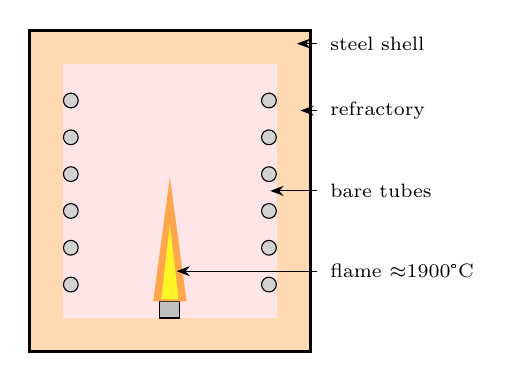
\begin{tikzpicture}[scale=0.85,font=\scriptsize,>=Stealth]
\fill[orange!30] (0,0) rectangle (4.2,4.8);\draw[very thick] (0,0) rectangle (4.2,4.8);\fill[red!10] (0.5,0.5) rectangle (3.7,4.3);
\foreach \y in {1.0,1.55,2.1,2.65,3.2,3.75}{\draw[fill=gray!35] (0.62,\y) circle (1.1mm);\draw[fill=gray!35] (3.58,\y) circle (1.1mm);}
\draw[fill=black!25] (1.95,0.5) rectangle (2.25,0.75);\fill[orange!70] (1.85,0.75)--(2.35,0.75)--(2.1,2.6)--cycle;\fill[yellow!85] (1.97,0.78)--(2.23,0.78)--(2.1,1.9)--cycle;
\node[anchor=west] at (4.35,4.6){steel shell};\draw[->] (4.3,4.6)--(4.0,4.6);\node[anchor=west] at (4.35,3.6){refractory};\draw[->] (4.3,3.6)--(4.05,3.6);
\node[anchor=west] at (4.35,2.4){bare tubes};\draw[->] (4.3,2.4)--(3.6,2.4);\node[anchor=west] at (4.35,1.2){flame $\approx$1900\textdegree C};\draw[->] (4.3,1.2)--(2.2,1.2);
\end{tikzpicture}\\[2pt]{\scriptsize (a) firebox cross-section}
\end{minipage}\hfill
\begin{minipage}[b]{0.58\linewidth}\centering
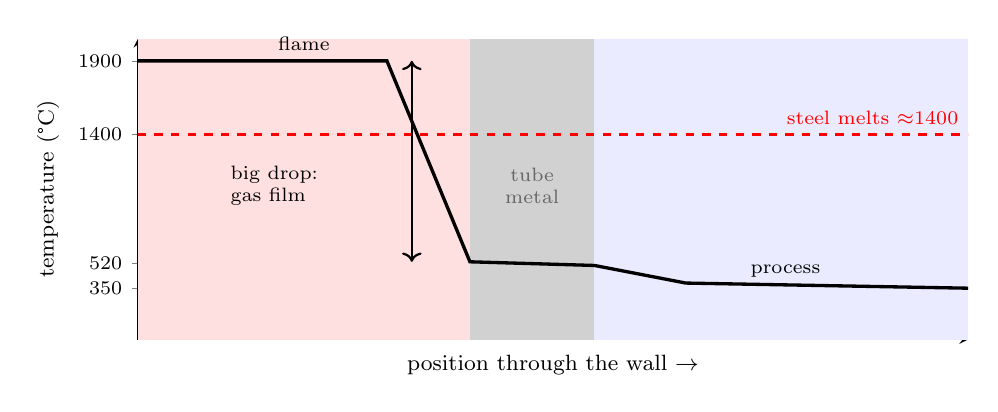
\begin{tikzpicture}\begin{axis}[width=\linewidth,height=5.4cm,xlabel={position through the wall $\rightarrow$},ylabel={temperature (\textdegree C)},xmin=0,xmax=10,ymin=0,ymax=2050,xtick=\empty,ytick={350,520,1400,1900},yticklabels={350,520,1400,1900},axis lines=left,clip=false,label style={font=\footnotesize},tick label style={font=\scriptsize}]
\fill[red!12] (axis cs:0,0) rectangle (axis cs:4,2050);\fill[black!18](axis cs:4,0) rectangle (axis cs:5.5,2050);\fill[blue!8] (axis cs:5.5,0) rectangle (axis cs:10,2050);
\addplot[dashed,red,very thick,domain=0:10,samples=2]{1400};\node[red,anchor=south east,font=\scriptsize] at (axis cs:10,1400){steel melts $\approx$1400};
\addplot[very thick,black] coordinates {(0,1900)(3,1900)(4,530)(5.5,505)(6.6,385)(10,350)};
\node[anchor=south,font=\scriptsize] at (axis cs:2,1905){flame};\node[align=center,black!60,font=\scriptsize] at (axis cs:4.75,1050){tube\\metal};\node[anchor=south,font=\scriptsize] at (axis cs:7.8,360){process};
\draw[<->,thick] (axis cs:3.3,1900)--(axis cs:3.3,530);\node[anchor=west,align=left,font=\scriptsize] at (axis cs:1.0,1050){big drop:\\gas film};
\end{axis}\end{tikzpicture}\\[2pt]{\scriptsize (b) temperature profile}
\end{minipage}
\caption{Why furnace tubes survive a 1900\,\textdegree C flame. (a) The radiant tubes hang BARE along the firebox walls, exposed to the flame; the refractory lines the WALLS (protecting the steel shell and re-radiating heat), not the tubes. (b) Almost the whole temperature drop falls across the outer gas film, so the tube metal sits near 520\,\textdegree C -- far below its melting point -- because the process fluid inside removes the heat as fast as it arrives. Lose the flow and the metal races toward the flame temperature.}\end{figure}

Two lessons: (1) the metallurgy is specified for the \textbf{tube-metal
temperature}, not the flame (carbon steel \textasciitilde400 \textdegree{}C, 9Cr-1Mo
\textasciitilde650 \textdegree{}C, cast HK/HP austenitics to \textasciitilde1000
\textdegree{}C); the firebox walls are protected by \textbf{refractory} lining, not
bare metal. (2) If the process flow STOPS or drops (pump trip, coking),
the heat is no longer removed and the tube temperature runs away in
\textbf{seconds} --- the tube ruptures. That is why a fired heater
carries a \textbf{low-flow trip} and the flux is capped: a hot tube with
no flow is the classic furnace failure.

\hypertarget{compressors-expanders--pressure-change}{%
\section{Compressors, expanders \& pressure
change}\label{compressors-expanders--pressure-change}}

Gas pressure change is governed by \emph{volumetric flow at suction} and
\emph{required pressure ratio} \texttt{r\ =\ P\_out/P\_in} --- not mass
flow. Because gas density falls as you compress, machine choice tracks
\textbf{actual inlet m\textsuperscript{3}/h} and \texttt{r}, then degrades to the next
type as flow rises or \texttt{r} falls. Treat every heuristic below as a
hypothesis: run the case in Choupo, read \texttt{W\_shaft} and discharge
T, and check you stayed inside the box.

\hypertarget{type-selection-1}{%
\subsection{TYPE SELECTION}\label{type-selection-1}}

\begin{longtable}[]{@{}>{\raggedright\arraybackslash}p{\dimexpr(\linewidth-10\tabcolsep)/5\relax}>{\raggedright\arraybackslash}p{\dimexpr(\linewidth-10\tabcolsep)/5\relax}>{\raggedright\arraybackslash}p{\dimexpr(\linewidth-10\tabcolsep)/5\relax}>{\raggedright\arraybackslash}p{\dimexpr(\linewidth-10\tabcolsep)/5\relax}>{\raggedright\arraybackslash}p{\dimexpr(\linewidth-10\tabcolsep)/5\relax}@{}}
\toprule\noalign{}
Type & Inlet flow (actual m\textsuperscript{3}/h) & r per body & Typical \(\eta\)\_poly & Why /
physics \\
\midrule\noalign{}
\endhead
\bottomrule\noalign{}
\endlastfoot
Fan / blower & 10\textsuperscript{3}--10\textsuperscript{6} & \textless1.1 (fan), \textless2 (blower) &
0.55--0.75 & Low \(\Delta\)p; cheap; r limited before it becomes a
"compressor" \\
Centrifugal & 1,700--340,000 & 1.5--3 per wheel, \textasciitilde10
multi-stage & 0.75--0.85 & Dynamic; smooth, oil-free, high flow; surge
limits turndown \\
Axial & \textgreater65,000 & 1.2--1.5 per stage & 0.80--0.88 & Highest
flow, best \(\eta\); narrow operating window \\
Reciprocating & \textless16,000 & up to 5--10 per stage & 0.75--0.90 &
Positive-displacement; best for high r, low flow, high P
(\textgreater200 bar) \\
Rotary screw & \textless5,000 & 3--4 (up to \textasciitilde8
oil-flooded) & 0.70--0.78 & Robust, dirty/wet gas, modest r; oil
carryover \\
\end{longtable}

\hypertarget{stages-ratio-per-stage--intercooling}{%
\subsection{Stages, ratio per stage \&
intercooling}\label{stages-ratio-per-stage--intercooling}}

Split \texttt{r} across N stages with \textbf{equal ratio per stage}
\texttt{r\_stage\ =\ r\^{}(1/N)}, kept to \textbf{\textasciitilde2--4}
(cap \textasciitilde4 for recips, \textasciitilde3 for centrifugals).
Equal ratios minimise total shaft work and equalise per-stage discharge
T. The driver of staging is the \textbf{discharge-temperature limit}:
keep \texttt{T\_out\ \(\lesssim\)\ 150--175\ \textdegree{}C} (lube-oil coking, gasket and
rod-packing life; \textasciitilde200 \textdegree{}C absolute ceiling). Adiabatic
\texttt{T\_out\ =\ T\_in\textperiodcentered{}r\_stage\^{}((\(\gamma\)\textminus{}1)/(\(\gamma\)\(\eta\)))}, so a single jump
from 1\(\rightarrow\)16 bar on a \(\gamma\)\(\approx\)1.3 gas blows past 250 \textdegree{}C --- unacceptable.
\textbf{Intercool back to \textasciitilde40 \textdegree{}C} between stages: this
cuts the next stage\textquotesingle s volumetric work (you compress
colder, denser gas) and typically saves 10--20 \% total power for
\texttt{r\ \textgreater{}\ \textasciitilde{}5}. Pair an intercooler with
a knock-out drum --- cooling condenses water/heavy ends that would erode
the next stage. In Choupo, model each stage as a \texttt{compressor}
(W\_shaft + \(\eta\)) feeding a cooler + flash; cooling-water or chilled-water
utilities by T-level supply the intercooler duty.

\hypertarget{efficiency-surge--turndown}{%
\subsection{Efficiency, surge \&
turndown}\label{efficiency-surge--turndown}}

Quote \textbf{polytropic} efficiency (0.75--0.85 centrifugal, up to 0.88
axial) for design --- it is path-independent and additive across stages,
whereas isentropic \(\eta\) drifts with \texttt{r}. Multiply by
\textasciitilde0.95 mechanical to get brake power. Dynamic machines
\textbf{surge} at \textasciitilde60--70 \% of design flow (flow
reversal, violent oscillation), so usable \textbf{turndown is only to
\textasciitilde70 \%} without recycle/anti-surge; recips turn down to
\textasciitilde25 \% via clearance pockets or speed. Size with
\textasciitilde10 \% flow margin above the surge line.

\hypertarget{when-an-expander-pays-back}{%
\subsection{When an expander pays
back}\label{when-an-expander-pays-back}}

If a hot, high-P stream must be let down (\(\ge\)3--4 bar drop, \(\ge\)a few hundred
kW recoverable), replace the throttle valve with a
\textbf{turbo-expander} (model as \texttt{turbine}, W\_shaft +
\(\eta\)\(\approx\)0.80--0.85). Recovered shaft work directly drives a generator or a
companion compressor (common in refrigeration, FCC flue-gas, cryogenic
N\textsubscript{2}). The trade-off: expansion chills the stream (Joule--Thomson + work
extraction), so verify you don\textquotesingle t cross a dew/freeze
point --- a glass-box run shows the outlet T before you commit hardware.

\hypertarget{drivers-electric-motors-steam--gas-turbines}{%
\section{Drivers: electric motors, steam \& gas
turbines}\label{drivers-electric-motors-steam--gas-turbines}}

A pump or compressor is only as available as the machine that turns it.
The \emph{driver} is a separate selection from the
hydraulic/thermodynamic duty: pick it by shaft power, by what HP steam
or fuel gas the plant already has, and by what must keep running when
the grid trips. In Choupo the rotating unit carries
\texttt{W\_shaft\ +\ eta}; the driver question is \emph{where that shaft
power comes from} and at what reliability.

\textbf{Rule --- electric motor is the default below
\textasciitilde0.5--1 MW.} Standard TEFC induction motors are cheap,
compact, \textasciitilde93--97\% efficient, and need no auxiliaries. WHY
the ceiling: above \textasciitilde1 MW you move to medium-voltage (4.16
kV+) switchgear and the incremental
\(/kW of motor + variable-frequency drive (VFD) climbs, while a steam turbine that *also* lets HP steam down to a useful level starts to win on combined steam-balance economics. Hypothesis to run: size the motor at ~110--125% of `W_shaft/eta_pump` (service factor + driver-train losses), then check the plant power bill at ~
\)0.06--0.10/kWh.

\textbf{Rule --- steam turbine when HP steam exists, for very large
duty, or as a trip-proof spare.} A back-pressure turbine taking HP\(\rightarrow\)MP/LP
steam "pays" for shaft work by letting steam down a pressure level you
needed anyway --- marginal cost is only the lost power-generation
credit, so isentropic efficiency of 65--80\% (small) to
\textasciitilde85\% (large) is acceptable. A condensing turbine (exhaust
to \textasciitilde0.1 bar) maximises work but dumps \textasciitilde2
MJ/kWh of latent heat to cooling water. Critically, a steam turbine
keeps spinning on a grid blackout, so the boiler-feedwater pump and
reactor-quench pump are classically \emph{steam-turbine-driven spares}
on a motor-driven main (or vice-versa).

\textbf{Rule --- gas turbine only for very large power + heat (combined
heat-and-power).} Below \textasciitilde5 MW the heat-rate and capital
rarely justify it; above \textasciitilde10--15 MW a gas turbine with a
heat-recovery steam generator delivers shaft power \emph{and} the HP
steam header --- the cogeneration case Choupo models with steam
utilities by T-level.

\begin{longtable}[]{@{}>{\raggedright\arraybackslash}p{\dimexpr(\linewidth-10\tabcolsep)/5\relax}>{\raggedright\arraybackslash}p{\dimexpr(\linewidth-10\tabcolsep)/5\relax}>{\raggedright\arraybackslash}p{\dimexpr(\linewidth-10\tabcolsep)/5\relax}>{\raggedright\arraybackslash}p{\dimexpr(\linewidth-10\tabcolsep)/5\relax}>{\raggedright\arraybackslash}p{\dimexpr(\linewidth-10\tabcolsep)/5\relax}@{}}
\toprule\noalign{}
Driver & Sweet-spot power & Efficiency & Pick it WHEN & Watch-out \\
\midrule\noalign{}
\endhead
\bottomrule\noalign{}
\endlastfoot
Electric motor (fixed-speed) & \textless{} 0.5 MW & 93--97\% &
small/medium duty, throttled or constant flow & dumps control margin
across a valve \\
Electric motor + VFD & 0.1--5 MW & 90--95\% (incl. drive) & flow varies
\textgreater{} \(\pm\)20\% & drive cost, harmonics, \textasciitilde3--5\%
drive loss \\
Back-pressure steam turbine & 0.5--15 MW & 65--85\% isentropic & HP
steam available, want MP/LP let-down & power tied to steam demand \\
Condensing steam turbine & 1--30 MW & 70--85\% isentropic & large duty,
run-on-trip spare & condenser + cooling-water latent load \\
Gas turbine (CHP) & \textgreater{} 10 MW & 30--40\% (\(\approx\)80\% w/ HRSG) &
huge power + process steam & fuel-gas spec, NOx, hot-day derate \\
\end{longtable}

\textbf{Rule --- variable speed beats throttling when flow turndown
exceeds \textasciitilde\(\pm\)20\%.} Power scales \textasciitilde speed\textsuperscript{3} on a
centrifugal machine, so trimming flow by slowing the driver saves far
more than burning the surplus head across a control valve. WHY not
always: a VFD adds \textasciitilde3--5\% standing loss and capital, so
for near-constant flow a fixed-speed motor + control valve is cheaper
and simpler.

\textbf{Rule --- spare to n+1 on critical service.} Install one extra
parallel machine (e.g. 3\(\times\)50\% pumps, run 2) so a single failure or
maintenance outage does not stop the plant; mix drivers (one motor, one
turbine) so a \emph{common-mode} loss --- grid or steam --- still leaves
one runner. Verify by toggling a unit offline and re-running the
flowsheet: does the remaining capacity still meet duty?

\hypertarget{fluid-transport-line-sizing--hydraulics}{%
\section{Fluid transport, line sizing \&
hydraulics}\label{fluid-transport-line-sizing--hydraulics}}

Moving fluid costs capital (pipe + driver) and power (friction). Every
rule below trades a \emph{bigger pipe / lower velocity} (more steel,
less \(\Delta\)P, less erosion) against a \emph{smaller pipe / higher velocity}
(cheap, but pumping power and noise climb as \textasciitilde v\textsuperscript{2}\textperiodcentered{}\textsuperscript{8}). Pick
the driver by \textbf{pressure-ratio first, then flow}.

\hypertarget{driver-selection-by-pressure-ratio}{%
\subsection{Driver selection by pressure
ratio}\label{driver-selection-by-pressure-ratio}}

\begin{longtable}[]{@{}>{\raggedright\arraybackslash}p{\dimexpr(\linewidth-8\tabcolsep)/4\relax}>{\raggedright\arraybackslash}p{\dimexpr(\linewidth-8\tabcolsep)/4\relax}>{\raggedright\arraybackslash}p{\dimexpr(\linewidth-8\tabcolsep)/4\relax}>{\raggedright\arraybackslash}p{\dimexpr(\linewidth-8\tabcolsep)/4\relax}@{}}
\toprule\noalign{}
Service & \(\Delta\)p / ratio & Pick & Why (glass-box) \\
\midrule\noalign{}
\endhead
\bottomrule\noalign{}
\endlastfoot
Incompressible liquid & any head & \textbf{Pump} (centrifugal
\textless\textasciitilde3500 m, recip/PD for low-flow high-head,
viscous, or metering) & \(\rho\)\(\approx\)const \(\rightarrow\) head, not ratio, is the variable \\
Gas, \(\Delta\)P \textless{} 0.03 bar & ratio \(\approx\)1.0--1.03 & \textbf{Fan} & \(\rho\)
change negligible, treat as incompressible \\
Gas, 0.03--3 bar & ratio \textasciitilde1.03--1.3 & \textbf{Blower} (one
stage) & mild heating, no intercool \\
Gas, ratio \textgreater{} \textasciitilde1.3 & up to
\textasciitilde3--4/stage & \textbf{Compressor} (centrifugal; recip for
very high ratio/low flow) & T\_out rises with ratio\^{}((\(\gamma\)\textminus{}1)/\(\gamma\)) \(\rightarrow\)
\textbf{stage + intercool if total ratio \textgreater{}
\textasciitilde4} \\
\end{longtable}

Multi-stage rule: keep per-stage ratio \(\approx\) (total ratio)\^{}(1/N) so each
stage does equal work and discharge T stays below
\textasciitilde150--200 \textdegree{}C (lubricant/material limit). See
\texttt{tutorials/steady/rotating/compressor01\_air} and the multi-stage
logic behind \texttt{compressorTurbine01\_turbo\_booster}; pumps in
\texttt{pump01\_water} / \texttt{pump02\_pressure\_spec}.

\hypertarget{recommended-superficial-velocities}{%
\subsection{Recommended superficial
velocities}\label{recommended-superficial-velocities}}

\begin{longtable}[]{@{}>{\raggedright\arraybackslash}p{\dimexpr(\linewidth-6\tabcolsep)/3\relax}>{\raggedright\arraybackslash}p{\dimexpr(\linewidth-6\tabcolsep)/3\relax}>{\raggedright\arraybackslash}p{\dimexpr(\linewidth-6\tabcolsep)/3\relax}@{}}
\toprule\noalign{}
Line / service & v (m/s) & Note \\
\midrule\noalign{}
\endhead
\bottomrule\noalign{}
\endlastfoot
Pump \textbf{suction} (liquid) & 0.5--1.5 & low to protect NPSH;
\(\Delta\)P\_suction is precious \\
Pump \textbf{discharge} / process liquid & 1.5--3 (up to
\textasciitilde4.5) & economic optimum; \textgreater4 erosion-corrosion
risk \\
Liquid, viscous/slurry & 0.5--1.5 & keep below settling; above abrasion
limit \\
Gas / vapour, atmospheric--low P & 15--30 & density-limited \\
Gas, high pressure & 10--20 & \(\rho\) high \(\rightarrow\) same \(\rho\)v\textsuperscript{2} at lower v \\
Steam (sat./superheat) & 20--40 (to 60) & erosion + wet-steam
wire-drawing \\
Two-phase / flashing & 10--25 & avoid slug/annular; check \(\rho\)v\textsuperscript{2}
\textless{} \textasciitilde6000 kg/m\textperiodcentered{}s\textsuperscript{2} \\
\end{longtable}

The economic optimum tracks \textbf{constant \(\rho\)v\textsuperscript{2}} (kinetic head), which
is why dense fluids run slower. A quick screen: \textbf{v\_econ \(\approx\) 2 m/s
liquid, 20 m/s gas}, then verify \(\Delta\)P in
\texttt{tutorials/steady/hydraulics/pipe01\_water\_line}.

\hypertarget{economic-pipe-diameter--ux3b4p-budget}{%
\subsection{Economic pipe diameter \& \(\Delta\)P
budget}\label{economic-pipe-diameter--ux3b4p-budget}}

\begin{itemize}
\tightlist
\item
  Rough optimum: \textbf{D\_econ \(\approx\) 0.26\textperiodcentered{}\(\dot{m}\)\^{}0.5\textperiodcentered{}\(\rho\)\^{}\textminus{}0.37} (m, SI) for
  turbulent steel --- the balance of pipe capital vs pumping power.
\item
  \textbf{\(\Delta\)P budget:} liquid lines \textbf{0.2--0.5 bar per 100 m} (\(\approx\)0.5
  kPa/m); gas lines \textbf{0.1--0.2 kPa/m}; long pipelines push lower
  (0.05). Total pump head = static lift + friction + equipment +
  \textbf{control-valve allowance}.
\item
  \textbf{Control-valve \(\Delta\)P:} allocate the \emph{larger} of
  \textbf{20--33 \% of dynamic (friction) \(\Delta\)P} or
  \textbf{\textasciitilde0.7 bar (10 psi)}, so the valve keeps authority
  at high flow. Too little \(\rightarrow\) loop goes open-loop; too much \(\rightarrow\) wasted
  head.
\end{itemize}

\hypertarget{npsh-the-pump-killer}{%
\subsection{NPSH (the pump killer)}\label{npsh-the-pump-killer}}

Require \textbf{NPSH\_available \textminus{} NPSH\_required \(\ge\) 0.5--1 m} margin.
NPSH\_a = (P\_suction \textminus{} P\_vap)/\(\rho\)g + static head \textminus{} suction friction.
Levers: raise the suction vessel, fatten/shorten suction line (low v,
see table), subcool, or cut speed. Hot/near-boiling liquids (reboiler
bottoms, deaerator) are the classic cavitation traps --- design suction
generously.

\textbf{Always run it:} these are \emph{hypotheses} --- size the line,
then let Choupo print the actual \(\Delta\)P, T\_out and head so the chosen
velocity and driver prove themselves.

\hypertarget{control-valves-pressure-letdown--choking}{%
\section{Control valves, pressure letdown \&
choking}\label{control-valves-pressure-letdown--choking}}

A control valve is a deliberate, adjustable restriction --- you spend
pressure to gain control. Two questions fix the hardware: which valve
body and trim, and whether the drop is so large it CHOKES.

\begin{longtable}[]{@{}>{\raggedright\arraybackslash}p{\dimexpr(\linewidth-6\tabcolsep)/3\relax}>{\raggedright\arraybackslash}p{\dimexpr(\linewidth-6\tabcolsep)/3\relax}>{\raggedright\arraybackslash}p{\dimexpr(\linewidth-6\tabcolsep)/3\relax}@{}}
\toprule\noalign{}
Valve & Rangeability & Use when \\
\midrule\noalign{}
\endhead
\bottomrule\noalign{}
\endlastfoot
Globe (single / multi-stage trim) & 20--50:1 & throttling --- the
default; high \(\Delta\)P; anti-cavitation / low-noise trim available \\
Ball / segmented & 100--300:1 & high rangeability, slurries,
on-off-to-throttle \\
Butterfly & 20--50:1 & large lines, low \(\Delta\)P, cheap \\
\end{longtable}

Pick the \textbf{inherent characteristic} to linearise the loop:
\textbf{equal-percentage} when most of the system \(\Delta\)P is elsewhere (the
common default --- valve gain rises with flow to offset its falling \(\Delta\)P);
\textbf{linear} when valve \(\Delta\)P dominates; \textbf{quick-opening} for
on-off. Liquid sizing (non-flashing): Q = Cv\textperiodcentered{}sqrt(\(\Delta\)P/SG); size for
\textasciitilde80\% open at max flow and \textasciitilde20\% at min, so
the plug never sits on the seat (no control) or wide open (no margin).

\textbf{Choking --- the answer to "is a big letdown done in one stage?"}

\begin{figure}[h]\centering
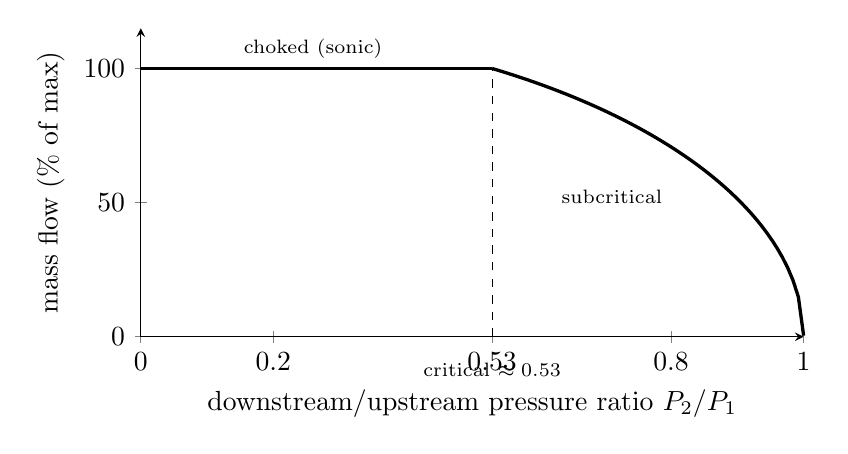
\begin{tikzpicture}\begin{axis}[width=10cm,height=5.5cm,xlabel={downstream/upstream pressure ratio $P_2/P_1$},ylabel={mass flow (\% of max)},xmin=0,xmax=1,ymin=0,ymax=115,xtick={0,0.2,0.53,0.8,1},axis lines=left,clip=false]
\addplot[very thick,black,domain=0:0.53,samples=2]{100};\addplot[very thick,black,domain=0.53:1,samples=60]{100*sqrt((1-x*x)/(1-0.53*0.53))};
\draw[dashed] (axis cs:0.53,0)--(axis cs:0.53,100);\node[anchor=south] at (axis cs:0.26,100){\scriptsize choked (sonic)};\node[anchor=west] at (axis cs:0.62,52){\scriptsize subcritical};\node[anchor=north] at (axis cs:0.53,-6){\scriptsize critical $\approx 0.53$};
\end{axis}\end{tikzpicture}\caption{Gas flow through a valve vs the pressure ratio. Below the critical ratio ($\approx0.53$ for air) the flow chokes -- sonic at the vena contracta -- and mass flow stops rising as $P_2$ falls; the surplus pressure drop becomes noise and erosion.}\end{figure}

For a GAS, flow does NOT keep rising as you drop the downstream
pressure. Once the pressure ratio falls below the \textbf{critical
ratio} --- r\_c = {[}2/(\(\gamma\)+1){]} raised to {[}\(\gamma\)/(\(\gamma\)\textminus{}1){]}, \(\approx\) \textbf{0.5
for most gases} (0.53 for air) --- the velocity at the vena contracta
reaches the speed of sound and the valve \textbf{CHOKES}: mass flow
saturates and the surplus \(\Delta\)P is dumped as \textbf{noise (often
\textgreater{} 110 dB), vibration and erosion}. Discharging 50 bar \(\rightarrow\) 1
atm is a ratio of 0.02, i.e. deeply choked.

So a single standard valve CAN pass the flow, but across a deeply choked
drop it screams, erodes its trim and shakes the pipe --- which is why a
large letdown is usually \textbf{staged}:

\begin{longtable}[]{@{}>{\raggedright\arraybackslash}p{\dimexpr(\linewidth-4\tabcolsep)/2\relax}>{\raggedright\arraybackslash}p{\dimexpr(\linewidth-4\tabcolsep)/2\relax}@{}}
\toprule\noalign{}
Letdown situation & Do this \\
\midrule\noalign{}
\endhead
\bottomrule\noalign{}
\endlastfoot
Small gas \(\Delta\)P, sub-critical & one globe valve \\
Large gas \(\Delta\)P, choked & multi-stage / labyrinth trim, or valves in
series, + a downstream silencer (each stage takes a sub-critical
drop) \\
Liquid, P\textsubscript{2} \textgreater{} Pvap & standard trim \\
Liquid, P\textsubscript{2} \textless{} Pvap (flashing) & the liquid flashes/cavitates
and imploding bubbles pit the trim --- use anti-cavitation (multi-step)
trim, harden it, or flash on purpose into a drum \\
\end{longtable}

Rule of thumb: stage it when the predicted noise exceeds
\textasciitilde85--90 dBA or the trim-exit velocity is high. The
glass-box check: drop the pressure across a \texttt{valve} in Choupo and
read the outlet T and phase --- a flashing liquid shows up as a vapour
fraction at the outlet before you ever buy the trim.

\hypertarget{refrigeration--vacuum-systems}{%
\section{Refrigeration \& vacuum
systems}\label{refrigeration--vacuum-systems}}

Cold and vacuum are \emph{bought power}. Both reject heat or pull gas
against the ambient, so the design instinct is the same: \textbf{climb
only as far down the ladder as the duty forces you, because every rung
multiplies the shaft work.}

\hypertarget{refrigeration--pick-the-warmest-level-that-works}{%
\subsection{Refrigeration --- pick the warmest level that
works}\label{refrigeration--pick-the-warmest-level-that-works}}

Cooling water (CW) leaves a tower at \textasciitilde30 C and can chill a
process stream to \textasciitilde35-40 C (10 C approach). The moment you
need a process temperature \textbf{below \textasciitilde40 C you have
left the free zone} and pay for a compressor. The reason is the
reverse-Carnot ceiling: ideal COP = T\_cold/(T\_hot\textminus{}T\_cold). Reject to
40 C cooling water and the COP collapses as the cold level drops --- so
shaft work per unit of cooling \emph{rises} the colder you go.

\begin{longtable}[]{@{}>{\raggedright\arraybackslash}p{\dimexpr(\linewidth-10\tabcolsep)/5\relax}>{\raggedright\arraybackslash}p{\dimexpr(\linewidth-10\tabcolsep)/5\relax}>{\raggedright\arraybackslash}p{\dimexpr(\linewidth-10\tabcolsep)/5\relax}>{\raggedright\arraybackslash}p{\dimexpr(\linewidth-10\tabcolsep)/5\relax}>{\raggedright\arraybackslash}p{\dimexpr(\linewidth-10\tabcolsep)/5\relax}@{}}
\toprule\noalign{}
Cold level needed & Medium & Refrig. T (C) & Ideal COP (reject
\textasciitilde40 C) & Real shaft kW per kW cooling \\
\midrule\noalign{}
\endhead
\bottomrule\noalign{}
\endlastfoot
\textgreater{} 40 C & Cooling water & n/a & --- & \textasciitilde0 (pump
only) \\
5-15 C & Chilled water & \textasciitilde5 & \textasciitilde6 & 0.15-0.25
(4-7 kW/kW) \\
\textminus{}40 to 0 C & Ammonia / propane & \textminus{}35 & \textasciitilde2.5-3 & 0.30-0.45
(2-3 kW/kW) \\
\textminus{}70 to \textminus{}40 C & Propylene & \textminus{}45 & \textasciitilde2 & 0.45-0.55 \\
\textminus{}100 to \textminus{}70 C & Ethylene (cascade) & \textminus{}90 & \textasciitilde1.3 & 0.6-0.9
(\textasciitilde1.3 kW/kW) \\
\textless{} \textminus{}100 C & Ethylene/methane cascade & \textminus{}150 & \textless{} 1 &
\textgreater{} 1 \\
\end{longtable}

\textbf{Rule of thumb:} budget \textbf{\textasciitilde1 kW shaft per 3-5
kW of cooling} at the \textminus{}40 to 0 C levels, climbing past \textasciitilde1
kW/kW below \textminus{}100 C. A single-stage cycle is fine for a
\textasciitilde40-50 C lift; beyond that, \textbf{cascade} (ethylene
rejecting into propylene rejecting into CW) because one compressor over
a 5:1+ pressure ratio runs hot and inefficient. In Choupo the
refrigeration compressor is just a \texttt{compressor} (W\_shaft + eta)
feeding the cold side of an exchanger; the warm reject side is
\texttt{coolingWater}, so the power penalty appears explicitly in the
work ledger --- model it, don\textquotesingle t assume it.

\textbf{When to refrigerate (not before):} a low-temperature condenser
to recover a light product (C3/C2 overhead), a cold separator to hit a
vapour-loss spec, or a reactor that must run cold for selectivity.
Always ask first whether \textbf{higher pressure} buys the same
condensation at a CW level --- compressing the overhead is often cheaper
than chilling it.

\hypertarget{vacuum--match-the-pump-to-the-absolute-pressure}{%
\subsection{Vacuum --- match the pump to the absolute
pressure}\label{vacuum--match-the-pump-to-the-absolute-pressure}}

Vacuum distillation earns its keep when the bottoms would
\textbf{thermally crack or polymerise} at the atmospheric boiling point
(heat-sensitive: glycols, fatty acids, monomers, vacuum gas oil).
Dropping to \textbf{0.05-0.1 bar (40-75 mmHg)} can cut boiling points by
80-150 C, keeping the reboiler below the degradation limit and off the
high-T utilities (Dowtherm A / fired heaters). Below \textasciitilde0.1
bar the \textbf{column diameter balloons} (vapour density falls, so
allowable mass velocity drops); use low-pressure-drop structured
packing, not trays.

\begin{longtable}[]{@{}>{\raggedright\arraybackslash}p{\dimexpr(\linewidth-6\tabcolsep)/3\relax}>{\raggedright\arraybackslash}p{\dimexpr(\linewidth-6\tabcolsep)/3\relax}>{\raggedright\arraybackslash}p{\dimexpr(\linewidth-6\tabcolsep)/3\relax}@{}}
\toprule\noalign{}
Absolute pressure & Technology & Notes / WHY \\
\midrule\noalign{}
\endhead
\bottomrule\noalign{}
\endlastfoot
1-0.1 bar & Liquid-ring pump & Rugged, tolerates condensables; service
water sets the floor (\textasciitilde30-50 mmHg) \\
0.1-0.01 bar & Single-stage steam ejector & No moving parts, uses MP/HP
steam; cheap but steam-hungry \\
\textless{} 0.01 bar (to \textasciitilde1 mmHg) & 2-3 stage ejectors w/
intercondensers & Stages compound the ratio; condensers cut steam
load \\
Clean, deep, dry & Dry screw pump & Electric, no steam/water effluent;
higher capex, watch for fouling \\
\end{longtable}

Size ejector \textbf{motive steam by the air/leakage load}, not the
process vapour --- a few kg/h of inleak through flanges sets the bill,
so a tight column beats a big ejector.

\hypertarget{storage--intermediate-tanks}{%
\section{Storage \& intermediate
tanks}\label{storage--intermediate-tanks}}

Storage is inventory bought with steel: too little and a late truck or a
tripped upstream unit starves the plant; too much and you pay for
tankage, land, and a larger fire/spill exposure. Size by \textbf{days of
stock} tied to the \emph{logistics} of each stream, then pick a roof
that matches the volatility. Run the hypothesis in Choupo by feeding the
tank\textquotesingle s design flow into a flash drum at storage T,P and
watching the vapour fraction --- if \texttt{vf\ \textgreater{}\ 0} you
have a breathing/venting problem a cone roof cannot hold.

\textbf{Sizing by days of stock (the WHY = decoupling time-scale):}

\begin{itemize}
\tightlist
\item
  \textbf{Raw materials:} \textasciitilde{}\textbf{7-30 days}. The
  driver is delivery reliability and shipment size --- rail/marine
  (large parcels, long lead) push to 20-30 days; reliable pipeline or
  daily truck supply drops to 3-7. Hold enough that a missed delivery
  does not stop the reactor.
\item
  \textbf{Products:} \textasciitilde{}\textbf{7-30 days}, set by
  shipping cadence and demand swing. A monthly tanker means
  \textasciitilde30 days plus working heel; spot-truck sales need only a
  few days.
\item
  \textbf{Intermediate / surge:} \textbf{hours to \textasciitilde2
  days}. Purpose is to \emph{decouple} two units so a transient in one
  does not propagate. Rule of thumb: \textbf{5-15 min} of holdup for
  pump-suction/control surge, \textbf{0.5-2 days} between batch and
  continuous sections (e.g. a reactor feeding a continuous still). More
  surge = looser control coupling but slower composition response and
  more off-spec inventory if upstream drifts.
\end{itemize}

Tank \textbf{working volume} = days \(\times\) daily throughput, then divide by
the \textbf{fill fraction}: never design to the brim. \textbf{Fill
\textasciitilde85-90\%}, leaving \textbf{10-15\% ullage} for thermal
expansion (a 30 \textdegree{}C swing on a hydrocarbon adds \textasciitilde3-4
vol\%), foam, and high-level-alarm margin. Overfill is a top cause of
major releases (Buncefield), so the ullage is a safety budget, not
slack.

\textbf{Type selection (volatility \& pressure drive the roof):}

\begin{longtable}[]{@{}>{\raggedright\arraybackslash}p{\dimexpr(\linewidth-10\tabcolsep)/5\relax}>{\raggedright\arraybackslash}p{\dimexpr(\linewidth-10\tabcolsep)/5\relax}>{\raggedright\arraybackslash}p{\dimexpr(\linewidth-10\tabcolsep)/5\relax}>{\raggedright\arraybackslash}p{\dimexpr(\linewidth-10\tabcolsep)/5\relax}>{\raggedright\arraybackslash}p{\dimexpr(\linewidth-10\tabcolsep)/5\relax}@{}}
\toprule\noalign{}
Tank type & Best for & Pressure / vapour-pressure range & Typical size &
Why \\
\midrule\noalign{}
\endhead
\bottomrule\noalign{}
\endlastfoot
\textbf{Cone (fixed) roof} & Non-volatile liquids: water, heavy oils,
glycols, most products with RVP \textless{} \textasciitilde10 kPa &
Atmospheric, near-zero gauge & up to \textasciitilde10,000 m\textsuperscript{3} &
Cheapest; vapour space breathes in/out --- fine when
there\textquotesingle s little vapour to lose \\
\textbf{External floating roof} & Volatile liquids: gasoline, naphtha,
light solvents (RVP \textasciitilde10-80 kPa) & Atmospheric &
\textasciitilde1,000-100,000 m\textsuperscript{3} & Roof rides on the liquid \(\rightarrow\) \textbf{no
vapour space}, cuts breathing/standing losses by \textasciitilde95\% vs
cone roof; emissions + fire-risk reduction \\
\textbf{Internal floating roof} & Volatiles needing weather/rain
protection & Atmospheric & medium & Floating deck under a fixed roof ---
losses control plus debris exclusion \\
\textbf{Sphere (Hortonsphere)} & LPG, propane, butane, light ends &
\textasciitilde2-18 barg (vapour pressure \textgreater{} atm) &
\textasciitilde1,000-10,000 m\textsuperscript{3} & Sphere carries pressure with minimum
steel/area; even stress distribution \\
\textbf{Bullet (horizontal cylinder)} & Smaller pressurised stock: LPG,
NH\textsubscript{3}, light ends & \textasciitilde5-25 barg & \textless{}
\textasciitilde500 m\textsuperscript{3} & Cheaper than a sphere below
\textasciitilde200-500 m\textsuperscript{3}; easy to transport and mound \\
\end{longtable}

\textbf{The crossover rule:} if the stored fluid\textquotesingle s true
vapour pressure exceeds atmospheric at the \emph{hottest} expected
ambient (summer-skin \textasciitilde45 \textdegree{}C), it \textbf{cannot} sit in an
atmospheric tank --- it must go pressurised (sphere/bullet). Between
non-volatile and pressurised lives the floating-roof band, chosen to cut
working+breathing losses you would otherwise vent or send to a
flare/recovery unit. Always state the range and let throughput, RVP, and
emissions cost decide --- there is no single right tank.

\hypertarget{process-control--instrumentation-heuristics}{%
\section{Process control \& instrumentation
heuristics}\label{process-control--instrumentation-heuristics}}

A flowsheet that balances on paper still must hold steady against
disturbances. The Pareto question is not tuning --- it is \textbf{what
to pair with what}. Choupo\textquotesingle s \texttt{choupoCtrl} + PID
lets you test a pairing on a dynamic case before you trust it.
\textbf{Hypothesis to run:} step a disturbance in \texttt{ctrl01} and
watch whether your loop rejects it or fights another.

\textbf{Inventory first.} Control every inventory (level, pressure)
before any quality --- an unbounded inventory shuts the plant down.

\begin{longtable}[]{@{}>{\raggedright\arraybackslash}p{\dimexpr(\linewidth-6\tabcolsep)/3\relax}>{\raggedright\arraybackslash}p{\dimexpr(\linewidth-6\tabcolsep)/3\relax}>{\raggedright\arraybackslash}p{\dimexpr(\linewidth-6\tabcolsep)/3\relax}@{}}
\toprule\noalign{}
Controlled variable & Manipulate & Why \\
\midrule\noalign{}
\endhead
\bottomrule\noalign{}
\endlastfoot
Level (drum, sump, tank) & the OUTflow & self-regulating; never control
level by an inflow that sets production \\
Pressure (vapour) & vent / vapour outflow / condenser duty & fast; pins
the vapour inventory \\
Feed flow / throughput & the feed valve directly & the master production
handle \\
Reactor / column temperature & coolant or steam duty & the quality
proxy \\
Column composition & a sensitive tray TEMPERATURE & direct composition
is slow/expensive; tray T tracks it \\
\end{longtable}

\textbf{Tuning starting points.} Process PID is \textbf{mostly PI} ---
derivative amplifies noise, so add D only on slow, lag-dominated
(temperature) loops. Flow loops: fast and tight. Level loops:
loose/averaging (the tank is a buffer). Use the open-loop step (gain,
dead time \(\theta\), time constant \(\tau\)) with an IMC/\(\lambda\) rule rather than trial and
error.

\textbf{Structure beyond single loops.}

\begin{itemize}
\tightlist
\item
  \textbf{Cascade} when a fast inner disturbance exists (jacket-T inside
  reactor-T rejects coolant upsets early).
\item
  \textbf{Feedforward} when a disturbance is MEASURED (feed
  rate/composition) --- act before the error appears, trim with
  feedback.
\item
  \textbf{Ratio} to hold two streams in proportion (stoichiometry,
  reflux, fuel/air).
\item
  \textbf{Override / constraint} to ride a limit (max T, min level)
  safely.
\end{itemize}

\textbf{Pairing discipline:} pair each manipulated variable with the
controlled variable it affects most directly and with least interaction
(a near-1 relative gain). Two loops that fight oscillate --- the
glass-box dynamic run shows it at once. Keep DOF honest: one independent
manipulated variable per controlled variable, no more.

\textbf{Equipment-specific schemes.} Beyond single loops, each unit has
a conventional strategy.

\begin{figure}[h]\centering
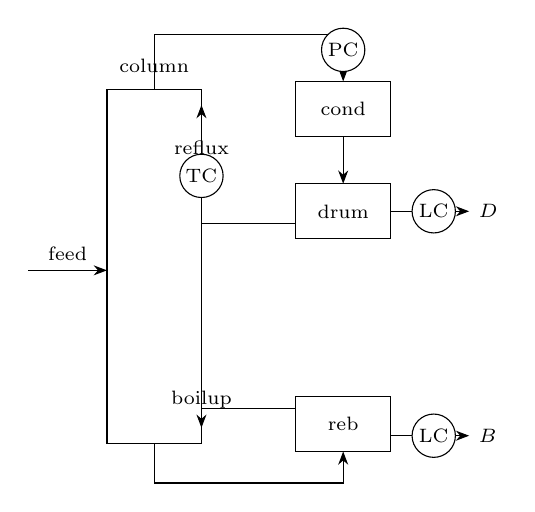
\begin{tikzpicture}[font=\scriptsize,>=Stealth,ctrl/.style={draw,circle,minimum size=5.5mm,inner sep=0,fill=white}]
\draw (0,0) rectangle (1.2,4.5); \node at (0.6,4.8){column};\draw[->] (-1,2.2)--(0,2.2) node[midway,above]{feed};\draw[->] (0.6,4.5)--(0.6,5.2)--(3,5.2)--(3,4.6);
\draw (2.4,3.9) rectangle (3.6,4.6); \node at (3,4.25){cond};\draw (2.4,2.6) rectangle (3.6,3.3); \node at (3,2.95){drum};\draw[->] (3,3.9)--(3,3.3);
\draw[->] (2.4,2.8)--(1.2,2.8)--(1.2,4.3) node[midway,above]{reflux};\draw[->] (3.6,2.95)--(4.6,2.95) node[right]{$D$};
\draw (2.4,-0.1) rectangle (3.6,0.6); \node at (3,0.25){reb};\draw[->] (0.6,0)--(0.6,-0.5)--(3,-0.5)--(3,-0.1);\draw[->] (2.4,0.45)--(1.2,0.45)--(1.2,0.2) node[midway,above]{boilup};\draw[->] (3.6,0.1)--(4.6,0.1) node[right]{$B$};
\node[ctrl] at (3,5.0){PC}; \node[ctrl] at (4.15,2.95){LC};\node[ctrl] at (1.2,3.4){TC}; \node[ctrl] at (4.15,0.1){LC};
\end{tikzpicture}\caption{A conventional distillation control scheme: pressure (PC) on the condenser, each level (LC) held by an outflow, composition by a sensitive tray temperature (TC). Five handles, five controlled variables -- the pairing is what makes it subtle.}\end{figure}

\emph{Distillation} is the hard one: a column has \textbf{five} handles
(condenser duty, distillate D, reflux L, boilup V, bottoms B) and
\textbf{five} things to hold (pressure, reflux-drum level, sump level, a
top and a bottom composition). Pressure is fixed first (condenser duty
or a vent). Each level MUST then be held by an OUTFLOW --- and the rule
is \textbf{control a level with the LARGER stream leaving that drum}: if
the reflux ratio R = L/D is high, reflux is the big stream, so hold
reflux-drum level with reflux and set D for composition (the "LV" vs
"DV" choice). Composition is inferred from a \textbf{sensitive tray
TEMPERATURE} (fast, cheap) instead of a slow analyser.
\textbf{Single-end} control (hold one composition, let the other float)
is the robust default; \textbf{dual-composition} control saves energy
but the two loops interact strongly (high relative gain) and usually
need decoupling --- which is exactly why students find column control
hard. \emph{Reactor:} temperature by coolant/steam duty, usually
\textbf{cascade} (jacket-T inner, reactor-T outer). \emph{Compressor:}
an \textbf{anti-surge} recycle loop keeps flow above the surge line.
\emph{Fired heater:} outlet T trims the fuel, with an air/fuel
\textbf{ratio} loop and a \textbf{low-flow trip} to protect the tubes.

\hypertarget{pressure-relief-flare--safety-basics}{%
\section{Pressure relief, flare \& safety
basics}\label{pressure-relief-flare--safety-basics}}

This is a Pareto orientation, not a safety course. The governing
standards are \textbf{API STD 520/521/526} (sizing, scenarios, devices)
and \textbf{API STD 537/NFPA 30}; treat the numbers below as
where-to-start hypotheses, then run the controlling case.

\textbf{When a device is mandatory.} \emph{Every} closed volume that can
be isolated and over-pressured needs an independent
overpressure-protection device --- no exceptions for "small" vessels.
The trigger is the credible-cause inventory, not size. A relief device
is the last line of defence: it must work with zero operator action and
zero instrument power, which is why a spring-loaded PSV (or rupture
disc) is preferred over an instrumented trip for the primary case.

\textbf{Set vs design pressure (the WHY).} Design pressure is set ABOVE
the maximum operating pressure so the PSV does not weep on normal
swings. Heuristic: \textbf{design P = max(1.1 \(\times\) operating P, operating P
+ 1.7 bar)}; for vessels under \textasciitilde7 barg the +1.7 bar floor
dominates, above it the +10\% rule does. The \textbf{PSV set pressure =
design pressure (MAWP)}. Code allows accumulation above set ---
typically \textbf{+10\%} for a single non-fire device, \textbf{+16\%}
for multiple devices, and \textbf{+21\%} for the fire case --- because
momentary overshoot during full relief is tolerable but permanent yield
is not.

\textbf{Sizing scenarios --- size for the worst credible single cause
(API 521).}

\begin{longtable}[]{@{}>{\raggedright\arraybackslash}p{\dimexpr(\linewidth-6\tabcolsep)/3\relax}>{\raggedright\arraybackslash}p{\dimexpr(\linewidth-6\tabcolsep)/3\relax}>{\raggedright\arraybackslash}p{\dimexpr(\linewidth-6\tabcolsep)/3\relax}@{}}
\toprule\noalign{}
Scenario & Typical controlling load & Why / note \\
\midrule\noalign{}
\endhead
\bottomrule\noalign{}
\endlastfoot
External fire & Wetted-area heat input \(\approx\) \textbf{43--70 kW/m\textsuperscript{2}} (q =
43.2\textperiodcentered{}F\textperiodcentered{}A\^{}0.82, SI) & Often controls vessels with large liquid
inventory; sets a large orifice \\
Blocked outlet & Full pump/compressor/feed flow at shut-in & Common
control case for pumped/compressed systems \\
Thermal expansion & Liquid trapped between two valves, heated & Tiny
relief (\textthreequarters{}"\(\times\)1") --- but mandatory; cheap to forget \\
Tube rupture (HX) & High-P side leaks to low-P side; full \(\Delta\)P flow & The
"2/3 rule": if low-side design P \textless{} 2/3 high-side, must
relieve \\
Control-valve failure / loss of cooling & Failed-open bypass,
reflux/condenser loss & Check fail-safe action of each valve \\
\end{longtable}

Size each, then \textbf{the largest required orifice wins}; pick the
next standard API-526 letter orifice (D through T).

\textbf{PSV vs rupture disc.}

\begin{longtable}[]{@{}>{\raggedright\arraybackslash}p{\dimexpr(\linewidth-6\tabcolsep)/3\relax}>{\raggedright\arraybackslash}p{\dimexpr(\linewidth-6\tabcolsep)/3\relax}>{\raggedright\arraybackslash}p{\dimexpr(\linewidth-6\tabcolsep)/3\relax}@{}}
\toprule\noalign{}
Device & Use when & Trade-off \\
\midrule\noalign{}
\endhead
\bottomrule\noalign{}
\endlastfoot
Spring PSV & Reclosing wanted; clean service & Reseals, testable; can
weep, can plug/foul \\
Rupture disc & Fast/large relief, fouling/corrosive, polymerising &
Non-reclosing (full loss of inventory); cheap \\
Disc + PSV in series & Corrosive service needing reseal & Disc
isolates/protects the PSV; best of both \\
\end{longtable}

\textbf{Disposal --- flare vs vent.} Vent to atmosphere only if the
relieved fluid is \textbf{non-toxic, non-flammable} at grade and the
discharge disperses safely (e.g. steam, air, inert). Flammable/toxic
streams route to a \textbf{closed flare header \(\rightarrow\) knockout drum \(\rightarrow\) flare},
sized so flare-tip exit velocity stays below
\textasciitilde{}\textbf{0.5 Mach} and grade-level radiation stays under
**\textasciitilde6.3 kW/m\textsuperscript{2}** at the fence (API 521). Choupo models the
relieved stream as a flash to header pressure; the \textbf{PSV-vent
enthalpy and flare duty appear in the first-law ledger}, so the energy
of blowdown is visible, not hidden.

\textbf{Spacing/segregation (Pareto).} Fired heaters and flares are
ignition sources --- keep \textbf{\textasciitilde15 m} from process
units handling flammables; locate control rooms and the flare
upwind/away. These setbacks are an insurance-grade default (IRI/GAP, API
521 \textsection{}5), refined later by a dispersion/QRA study.

\textbf{Governing standards --- go to the source; lives depend on it.}
This section is an orientation only; the binding requirements live in,
among others: pressure relief --- \textbf{API STD 520 \& 521}, tank
venting --- \textbf{API STD 2000}, overpressure protection ---
\textbf{ASME BPVC Section VIII} (UG-125+) and \textbf{Section I}
(boilers); relief-device specs --- \textbf{API STD 526}; flares ---
\textbf{API STD 521 \& 537}; process-safety management --- \textbf{OSHA
29 CFR 1910.119} and the \textbf{AIChE/CCPS} guideline series;
functional safety / SIS --- \textbf{IEC 61508 \& 61511}; hazard-study
method --- \textbf{IEC 61882 (HAZOP)}; flammable liquids ---
\textbf{NFPA 30}; electrical area classification --- \textbf{NFPA 70 /
IEC 60079}; facility siting --- \textbf{API RP 752/753}. Size and select
to the standard, then have it independently reviewed. See the Disclaimer
\& scope at the front of this guide.

\hypertarget{effluent-treatment--liquid--gaseous}{%
\section{Effluent treatment --- liquid \&
gaseous}\label{effluent-treatment--liquid--gaseous}}

Every flowsheet has a back door: the streams you do NOT sell. Design
them with the same care as the product train --- environmental limits
are \emph{legal} limits, and an untreated vent or outfall can shut a
plant down. \textbf{Hypothesis to run:} before sizing any treatment,
MINIMISE the load at source (recycle, substitution, leak reduction) ---
the cheapest effluent is the one never made.

\hypertarget{liquid-effluent-wastewater}{%
\subsection{Liquid effluent
(wastewater)}\label{liquid-effluent-wastewater}}

A train of increasing cost and specificity; stop when you meet the
discharge limit (typically COD, BOD, suspended solids, pH, oil \&
grease, specific toxics):

\begin{longtable}[]{@{}>{\raggedright\arraybackslash}p{\dimexpr(\linewidth-8\tabcolsep)/4\relax}>{\raggedright\arraybackslash}p{\dimexpr(\linewidth-8\tabcolsep)/4\relax}>{\raggedright\arraybackslash}p{\dimexpr(\linewidth-8\tabcolsep)/4\relax}>{\raggedright\arraybackslash}p{\dimexpr(\linewidth-8\tabcolsep)/4\relax}@{}}
\toprule\noalign{}
Stage & Removes & Typical numbers & Use when \\
\midrule\noalign{}
\endhead
\bottomrule\noalign{}
\endlastfoot
Equalisation + neutralisation & surges, pH & discharge pH 6--9; hours of
buffer & always first \\
API separator / DAF & free oil, solids & oil to \textless{} 10--50 mg/L
& oily / heavy-solids water \\
Biological (activated sludge) & BOD / COD & 85--98\% BOD removal; F/M
0.2--0.5 & biodegradable organics \\
Adsorption (GAC) / advanced oxidation & refractory toxics & polishing to
ppb & non-biodegradable, colour \\
Membrane (UF/RO) / evaporation & dissolved salts & water reuse,
zero-liquid-discharge & reuse or brine concentrate \\
\end{longtable}

WHY a train: each stage is cheap \emph{only} for what it targets ---
biology cannot take free oil, carbon is wasted on bulk BOD. Match the
stage to the contaminant.

\hypertarget{gaseous-effluent-air-emissions}{%
\subsection{Gaseous effluent (air
emissions)}\label{gaseous-effluent-air-emissions}}

\begin{longtable}[]{@{}>{\raggedright\arraybackslash}p{\dimexpr(\linewidth-6\tabcolsep)/3\relax}>{\raggedright\arraybackslash}p{\dimexpr(\linewidth-6\tabcolsep)/3\relax}>{\raggedright\arraybackslash}p{\dimexpr(\linewidth-6\tabcolsep)/3\relax}@{}}
\toprule\noalign{}
Pollutant & Control & Typical numbers \\
\midrule\noalign{}
\endhead
\bottomrule\noalign{}
\endlastfoot
Particulates & cyclone \(\rightarrow\) bag filter / ESP & baghouse to \textless{} 10
mg/m\textsuperscript{3}; cyclone only \textgreater{} 5--10 \textmu{}m \\
Acid gases (SOx, HCl) & wet / dry scrubber & 90--99\% removal; L/G 5--15
L/m\textsuperscript{3} \\
VOC, dilute \& high-flow & thermal / regenerative oxidiser & 95--99\%
destruction at 760--820 \textdegree{}C; RTO recovers \textasciitilde95\% heat \\
VOC, concentrated / valuable & condensation / carbon / absorption &
recover the solvent if it pays \\
NOx & low-NOx burner + SCR & SCR 80--90\% at 300--400 \textdegree{}C with ammonia \\
\end{longtable}

The master rule: \textbf{dilute-and-high-flow favours destruction
(oxidiser); concentrated-and-valuable favours recovery
(condense/absorb)} --- the same see-then-decide trade-off as everywhere
else. Choupo\textquotesingle s cyclone, absorber, and combustion duties
size the front end; the discharge limit is the spec and the local
regulation is the law (see \emph{Standards \& further reading}).

\hypertarget{cost-estimation--profitability}{%
\section{Cost estimation \&
profitability}\label{cost-estimation--profitability}}

Costing in Choupo is a \emph{post-processing pass}
(\texttt{CostingPass}, Guthrie/Turton models) feeding
\texttt{EconomicsPass} (see \texttt{optim05\_reactor\_npv}). The numbers
below are heuristics to be \emph{run and checked}, never final verdicts
--- accuracy depends entirely on the AACE estimate class.

\textbf{Capital (CAPEX).} Two routes, increasing in effort:

\begin{itemize}
\tightlist
\item
  \emph{Lang factor} --- fixed capital = Lang factor \(\times\) \(\Sigma\)(delivered
  equipment cost). Hypothesis to verify: a fluids plant lands near 4.7\(\times\);
  solids-handling near 3.1\(\times\); mixed 3.6\(\times\). The factor absorbs piping,
  instrumentation, civil, and indirects, so it is crude (\(\pm\)30-40\%) but
  fast.
\item
  \emph{Bare-module (Guthrie/Turton)} --- per-unit:
  \(C_{BM}=C_p^0\,F_{BM}\), with \(F_{BM}=(B_1+B_2 F_M F_P)\). Pressure
  (\(F_P\)) and material (\(F_M\)) multipliers are \emph{itemised}, so
  this is the glass-box default. Verify: a SS316 vessel at 30 bar shows
  \(F_{BM}\approx 5-7\) vs \textasciitilde3 for carbon steel at 1 bar.
\end{itemize}

\begin{longtable}[]{@{}>{\raggedright\arraybackslash}p{\dimexpr(\linewidth-6\tabcolsep)/3\relax}>{\raggedright\arraybackslash}p{\dimexpr(\linewidth-6\tabcolsep)/3\relax}>{\raggedright\arraybackslash}p{\dimexpr(\linewidth-6\tabcolsep)/3\relax}@{}}
\toprule\noalign{}
Item & Typical range & Why \\
\midrule\noalign{}
\endhead
\bottomrule\noalign{}
\endlastfoot
Lang factor (fluids) & 4.5-5.0 & Indirects dominate fluid plants \\
Lang factor (solids) & 3.0-3.6 & Less piping/instrumentation \\
Bare-module \(F_{BM}\) (CS, low-P) & 2.5-4.0 & Base installation
overhead \\
Six-tenths exponent \(n\) & 0.5-0.7 (\(\approx\)0.6) & Economy of scale on
area/volume \\
CEPCI escalation & index ratio & \textasciitilde600
(2019)\(\rightarrow\)\textasciitilde800 (2023) \\
Site/auxiliary uplift & +10-25\% & Grassroots vs battery-limit \\
\end{longtable}

\emph{Six-tenths rule:} \(C_2=C_1(S_2/S_1)^{0.6}\). Doubling capacity
raises cost only \textasciitilde52\% (2\^{}0.6) --- verify before sizing
a redundant train. \emph{CEPCI:}
\(C_{now}=C_{base}\,(I_{now}/I_{base})\); skipping a 4-year escalation
understates CAPEX \textasciitilde25\%.

\textbf{Operating cost (COM).} Rule of thumb (Turton):
\(COM \approx 0.18\,FCI + 2.73\,C_{OL} + 1.23(C_{UT}+C_{WT}+C_{RM})\).
Verify the dominant term:

\begin{longtable}[]{@{}>{\raggedright\arraybackslash}p{\dimexpr(\linewidth-6\tabcolsep)/3\relax}>{\raggedright\arraybackslash}p{\dimexpr(\linewidth-6\tabcolsep)/3\relax}>{\raggedright\arraybackslash}p{\dimexpr(\linewidth-6\tabcolsep)/3\relax}@{}}
\toprule\noalign{}
COM component & Typical share & Why \\
\midrule\noalign{}
\endhead
\bottomrule\noalign{}
\endlastfoot
Raw materials & 40-80\% & Usually dominant; selectivity is king \\
Utilities & 10-30\% & Steam/cooling/power --- pinch can cut 20-30\% \\
Labour + supervision & 5-15\% & Headcount \(\times\) shift factor 4.5 \\
Maintenance & 3-6\% of FCI & Wear-driven \\
\end{longtable}

Because raw materials dominate, a 1\% yield gain often beats any utility
optimisation --- test it against a pinch retrofit in the same case.

\textbf{Profitability.} Three lenses, never one:

\begin{itemize}
\tightlist
\item
  \emph{Payback period} (FCI / annual after-tax cash flow): attractive
  \textless3 yr, marginal 3-5 yr, suspect \textgreater5-6 yr. Ignores
  time value, so it is a screen only.
\item
  \emph{NPV} at a hurdle rate (10-15\% typical): positive \(\Rightarrow\)
  value-adding; verify sensitivity to discount rate and a 10-year
  horizon.
\item
  \emph{IRR/DCFROR}: the rate where NPV=0; want it 5-10 points above
  WACC. Below the hurdle even a short payback fails.
\end{itemize}

\textbf{Estimate class governs everything.} Report the band, not a
point:

\begin{longtable}[]{@{}>{\raggedright\arraybackslash}p{\dimexpr(\linewidth-8\tabcolsep)/4\relax}>{\raggedright\arraybackslash}p{\dimexpr(\linewidth-8\tabcolsep)/4\relax}>{\raggedright\arraybackslash}p{\dimexpr(\linewidth-8\tabcolsep)/4\relax}>{\raggedright\arraybackslash}p{\dimexpr(\linewidth-8\tabcolsep)/4\relax}@{}}
\toprule\noalign{}
AACE class & Maturity & Accuracy & Method \\
\midrule\noalign{}
\endhead
\bottomrule\noalign{}
\endlastfoot
Class 5 & 0-2\% & \textminus{}30/+50\% & Capacity-factored, six-tenths \\
Class 4 & 1-15\% & \textminus{}20/+30\% & Equipment-factored (Lang) \\
Class 3 & 10-40\% & \textminus{}15/+20\% & Bare-module / budget \\
Class 2 & 30-70\% & \textminus{}10/+15\% & Detailed, semi-quantitative \\
Class 1 & 50-100\% & \textminus{}5/+10\% & Definitive, quote-based \\
\end{longtable}

Quoting an NPV to four significant figures off a Class-5 estimate is the
classic glass-box failure: the \(\pm\)50\% CAPEX band swamps the answer.
Always run the case at both error bounds.

\hypertarget{materials-of-construction--mechanical-design}{%
\section{Materials of construction \& mechanical
design}\label{materials-of-construction--mechanical-design}}

Material choice is a \emph{climb-the-ladder} decision: start with the
cheapest metal that survives the duty, and step up only when corrosion
rate, chlorides, temperature, or hydrogen force you. Each rung is
roughly 1.5--4\(\times\) the cost of the one below, so an unjustified jump from
carbon steel to SS316 can double a vessel\textquotesingle s bare cost
(see Choupo\textquotesingle s Guthrie/Turton material-factor
\texttt{f\_M} in the costing pass; carbonSteel/SS304/SS316/aluminium are
the reference \texttt{data/materials/*.dat}).

\textbf{The selection ladder.} The governing rule of thumb is a target
corrosion rate \textbf{\textless{} 0.1 mm/yr} (\(\approx\) 5 mil/yr) for a 20-year
life; 0.1--0.5 mm/yr is tolerable with a fat allowance; above 0.5 mm/yr
step up.

\begin{longtable}[]{@{}>{\raggedright\arraybackslash}p{\dimexpr(\linewidth-6\tabcolsep)/3\relax}>{\raggedright\arraybackslash}p{\dimexpr(\linewidth-6\tabcolsep)/3\relax}>{\raggedright\arraybackslash}p{\dimexpr(\linewidth-6\tabcolsep)/3\relax}@{}}
\toprule\noalign{}
Service / limit & Pick & Why (the WHY) \\
\midrule\noalign{}
\endhead
\bottomrule\noalign{}
\endlastfoot
Dry hydrocarbons, steam, mild T \textless{} 400 \textdegree{}C & Carbon steel &
Cheapest; \textasciitilde0.1 mm/yr in benign duty \\
Dilute acids, oxidising, T \textless{} 60 \textdegree{}C, \textbf{chloride-free} &
SS304 & Cr\textsubscript{2}O\textsubscript{3} passive film; loses it to Cl\textsuperscript{\textminus} \\
Chlorides, dilute H\textsubscript{2}SO\textsubscript{4}, food/pharma & SS316 (2--3\% Mo) & Mo resists
pitting; PREN \(\approx\) 24 vs 18 \\
Hot chloride + tensile stress & Duplex 2205 / Ni alloy &
\textbf{Austenitic SCC} kills 304/316 \\
Strong HCl, wet Cl\textsubscript{2}, HF & Hastelloy C-276 / lined & General attack
defeats stainless \\
High-purity water, weight-critical & Aluminium & Cheap, light, but soft
\& low-T only \\
\end{longtable}

\textbf{Chlorides \& stress-corrosion (the silent killer).} Austenitic
304/316 suffer chloride \textbf{SCC} above \(\approx\) \textbf{60 \textdegree{}C} with tensile
stress and even ppm-level Cl\textsuperscript{\textminus} --- failures look like brittle cracking
with no wall loss, so a corrosion allowance does \emph{not} protect you.
Below 60 \textdegree{}C or for hot chlorides, jump to duplex (ferritic-austenitic,
immune) or nickel alloys. Pitting resistance scales with \textbf{PREN =
\%Cr + 3.3\textperiodcentered{}\%Mo + 16\textperiodcentered{}\%N} (304 \(\approx\) 18, 316 \(\approx\) 24, 2205 \(\approx\) 35).

\textbf{High-T creep \& hydrogen.} Carbon steel is creep-limited to \(\approx\)
\textbf{425 \textdegree{}C}; above this design stress collapses, so 1\textonequarter{}Cr--\textonehalf{}Mo, 9Cr,
or austenitics take over (relevant for fired-heater tubes and HiTec-salt
service to 535 \textdegree{}C). In H\textsubscript{2} at pressure, consult \textbf{Nelson curves}
(API 941): below the curve carbon steel is safe; above it, hydrogen
attacks carbides \(\rightarrow\) decarburisation and fissuring, demanding Cr-Mo
steels.

\textbf{Corrosion allowance.} Add \textbf{3.0 mm} standard (1.5 mm
benign, up to 6 mm aggressive). It is sacrificial metal, \emph{not} an
SCC or hydrogen fix.

\textbf{Wall thickness vs pressure.} Thin-wall (ASME VIII Div. 1):
\textbf{t = P\textperiodcentered{}R/(S\textperiodcentered{}E \textminus{} 0.6\textperiodcentered{}P) + CA}, with weld efficiency E = 0.85--1.0
and S the allowable stress (\(\approx\) 138 MPa for SS316 at moderate T). Design
pressure margin: \textbf{max(operating + 10\%, +1.7 bar)}; design
temperature: operating \textbf{+ 25 \textdegree{}C}. A minimum shell of
\textasciitilde6--8 mm is set by handling, not pressure.

\textbf{Aspect ratios.} Vertical process vessels and knockout drums:
\textbf{L/D \(\approx\) 3} (range 2--5) --- minimises wall metal at fixed volume
while giving disengaging height. Distillation columns run \textbf{L/D up
to 20--30}, capped by wind/seismic moment. Atmospheric storage tanks
favour \textbf{L/D \(\approx\) 0.5--1} (squat, cheap floor). Horizontal drums sit
at \textbf{L/D \(\approx\) 3--4}.

Glass-box check: re-run the Choupo sizing/costing pass swapping
\texttt{material\ carbonSteel;} \(\rightarrow\) \texttt{SS316;} and watch
\texttt{f\_M} and shell mass move; that is the cost of one rung.

\textbf{Corrosion allowance --- how many millimetres?} Wall thickness =
the pressure-stress thickness (from ASME) \textbf{plus a sacrificial
corrosion allowance}: CA = corrosion rate \(\times\) design life. Carbon steel
corroding at \textasciitilde0.1--0.25 mm/yr over a 20--25 year life
gives the familiar \textbf{3 mm} (1/8 in) allowance; severe service runs
to \textbf{6 mm}, clean/inert service to \textbf{0--1.5 mm}, and a
corrosion-resistant alloy needs \textbf{none} (it is chosen so the rate
is \textasciitilde0).

\begin{longtable}[]{@{}>{\raggedright\arraybackslash}p{\dimexpr(\linewidth-4\tabcolsep)/2\relax}>{\raggedright\arraybackslash}p{\dimexpr(\linewidth-4\tabcolsep)/2\relax}@{}}
\toprule\noalign{}
Corrosion rate & Verdict \\
\midrule\noalign{}
\endhead
\bottomrule\noalign{}
\endlastfoot
\textless{} 0.1 mm/yr & excellent --- carbon steel, 1.5--3 mm
allowance \\
0.1--0.5 mm/yr & acceptable with allowance + inspection \\
\textgreater{} 0.5 mm/yr & do NOT just thicken the steel --- upgrade the
alloy or line it \\
\end{longtable}

The rule: a corrosion allowance buys time, not safety --- above
\textasciitilde0.5 mm/yr the economics flip to a better material.

\textbf{Gaskets --- the small part that floods the floor.} A gasket
seals a flange by being squeezed between the faces; it must survive the
\textbf{pressure, the temperature, AND every fluid the joint ever sees
--- including cleaning.} Select by P--T--fluid:

\begin{longtable}[]{@{}>{\raggedright\arraybackslash}p{\dimexpr(\linewidth-6\tabcolsep)/3\relax}>{\raggedright\arraybackslash}p{\dimexpr(\linewidth-6\tabcolsep)/3\relax}>{\raggedright\arraybackslash}p{\dimexpr(\linewidth-6\tabcolsep)/3\relax}@{}}
\toprule\noalign{}
Gasket & P--T window & Use when \\
\midrule\noalign{}
\endhead
\bottomrule\noalign{}
\endlastfoot
Compressed fibre / PTFE sheet & to \textasciitilde20 bar,
\textasciitilde200 \textdegree{}C & low duty; PTFE for chemical resistance \\
Spiral-wound (metal + graphite/PTFE filler) & to \textasciitilde100+
bar, \textasciitilde450 \textdegree{}C+ & the workhorse for process flanges \\
Ring-joint (RTJ, solid metal) & very high P (\textgreater{} 100 bar) &
high-pressure gas, wellheads \\
\end{longtable}

The wetted material --- the winding and the filler --- must resist the
worst fluid, and the worst fluid is often \textbf{not} the product but
the \textbf{CLEANING} step. A gasket chosen only for cold wine will
corrode through during a \textbf{40 \textdegree{}C acid CIP wash}, and then the wine
runs out of the joint on the next batch --- a real and classic failure.
\textbf{Specify the gasket (and the bolt load) for the most aggressive
condition the joint ever sees, cleaning included}, never for normal
operation alone.

\hypertarget{standards--further-reading}{%
\section{Standards \& further
reading}\label{standards--further-reading}}

This guide distils the classic references below. For any real design go
to the primary source --- and for anything safety- or
environment-critical, the governing standard is the authority, not this
guide (see \emph{Disclaimer \& scope}).

\textbf{General process design \& heuristics}

\begin{itemize}
\tightlist
\item
  Turton, Shaeiwitz, Bhattacharyya \& Whiting, \emph{Analysis,
  Synthesis, and Design of Chemical Processes}, Prentice Hall.
\item
  Seider, Seader, Lewin \& Widagdo, \emph{Product and Process Design
  Principles}, Wiley.
\item
  Sinnott \& Towler, \emph{Chemical Engineering Design} (Coulson \&
  Richardson, Vol. 6), Butterworth-Heinemann.
\item
  Green \& Perry, \emph{Perry\textquotesingle s Chemical
  Engineers\textquotesingle{} Handbook}, McGraw-Hill.
\item
  Douglas, \emph{Conceptual Design of Chemical Processes}, McGraw-Hill.
\item
  Branan, \emph{Rules of Thumb for Chemical Engineers}; Walas,
  \emph{Chemical Process Equipment}.
\end{itemize}

\textbf{By topic}

\begin{itemize}
\tightlist
\item
  Heat integration / pinch --- Smith, \emph{Chemical Process Design and
  Integration}, Wiley; Kemp, \emph{Pinch Analysis and Process
  Integration}.
\item
  Distillation --- Kister, \emph{Distillation Design} \&
  \emph{Distillation Operation}, McGraw-Hill.
\item
  Heat transfer --- Kern, \emph{Process Heat Transfer}; \textbf{TEMA}
  standards.
\item
  Reactors --- Fogler, \emph{Elements of Chemical Reaction Engineering};
  Levenspiel, \emph{Chemical Reaction Engineering}.
\item
  Membranes --- Baker, \emph{Membrane Technology and Applications},
  Wiley.
\item
  Materials / corrosion --- \textbf{NACE/AMPP} standards; \textbf{API RP
  571} (damage mechanisms).
\item
  Effluent --- Metcalf \& Eddy, \emph{Wastewater Engineering};
  \textbf{US EPA} and \textbf{EU Industrial Emissions Directive (BAT /
  BREF)} guidance.
\end{itemize}

\textbf{Safety \& environmental standards --- binding, not optional}

\begin{itemize}
\tightlist
\item
  Pressure relief \& venting --- \textbf{API STD 520 / 521 / 526 /
  2000}; \textbf{ASME BPVC Sec. VIII \& I}.
\item
  Flares --- \textbf{API STD 521 / 537}.
\item
  Process-safety management --- \textbf{OSHA 29 CFR 1910.119};
  \textbf{AIChE CCPS} guideline series.
\item
  Functional safety / SIS --- \textbf{IEC 61508 / 61511}; HAZOP ---
  \textbf{IEC 61882}.
\item
  Flammables --- \textbf{NFPA 30}; electrical area classification ---
  \textbf{NFPA 70 / IEC 60079}.
\item
  Emissions \& discharge --- the local regulator\textquotesingle s
  limits (e.g. \textbf{US EPA}, \textbf{EU IED / BAT-BREF}).
\end{itemize}

\hypertarget{equipment-selection-at-a-glance}{%
\section{Equipment selection at a
glance}\label{equipment-selection-at-a-glance}}

\hypertarget{equipment-selection-at-a-glance-1}{%
\section{Equipment selection at a
glance}\label{equipment-selection-at-a-glance-1}}

This one-page table is the \emph{index of bets} --- each row is a duty
you will face, the default pick, the one-line reason, and the range to
start from. Treat every "typical number" as a hypothesis to verify by
running the linked Choupo case. When two picks compete, the table gives
the \textbf{default}; the section explains the crossover.

\begin{longtable}[]{@{}>{\raggedright\arraybackslash}p{\dimexpr(\linewidth-8\tabcolsep)/4\relax}>{\raggedright\arraybackslash}p{\dimexpr(\linewidth-8\tabcolsep)/4\relax}>{\raggedright\arraybackslash}p{\dimexpr(\linewidth-8\tabcolsep)/4\relax}>{\raggedright\arraybackslash}p{\dimexpr(\linewidth-8\tabcolsep)/4\relax}@{}}
\toprule\noalign{}
Duty / situation & Pick this & Because & Typical numbers \\
\midrule\noalign{}
\endhead
\bottomrule\noalign{}
\endlastfoot
Overall flowsheet structure & Reactor \(\rightarrow\) separation \(\rightarrow\) recycle, with a
purge on any loop that accumulates inerts & The "onion": fix conversion
+ recycle before heat/utilities; purge bleeds what recycle would
otherwise trap & Purge loses 1--5 \% of recycle; target recycle so
single-pass conversion \(\neq\) overall conversion \\
Equilibrium-limited reaction & Push reactor to \textasciitilde90--95 \%
of equilibrium, recycle the rest & Last few \% of approach costs
disproportionate volume; recycle is cheaper than oversizing &
Single-pass X = 0.6--0.9; overall X \textgreater{} 0.99 via recycle \\
Fast liquid-phase reaction, high conversion & PFR (or CSTR-in-series) &
Plug flow needs least volume for a given conversion; back-mixing
penalises high X & PFR vol \(\approx\) 1/3--1/2 of one CSTR at X = 0.9 \\
Autocatalytic, biological, solids-laden, or strong heat-removal duty &
CSTR (or CSTR train) & Back-mixing dilutes feed, eases T control and
solids handling & 3--4 CSTRs in series \(\approx\) PFR; \(\tau\) set by k and target X \\
Gas-phase catalytic reaction & Packed-bed (PFR model) & Heterogeneous
catalyst + plug flow; watch \(\Delta\)P across bed & Superficial gas 0.3--1 m/s;
bed \(\Delta\)P a few \% of P \\
Separate close-boiling liquids & Distillation & Cheapest workhorse
whenever relative volatility allows & Viable for \(\alpha\) \textgreater{}
\textasciitilde1.05; easy for \(\alpha\) \textgreater{} 1.5 \\
Distillation column operating point & Reflux R = 1.1--1.3 \(\times\) R\_min &
Optimum trades reflux (energy) vs trays (capital); flat-bottomed cost
curve & R/R\_min \(\approx\) 1.1--1.3; N \(\approx\) 2--2.5 \(\times\) N\_min \\
Heat-sensitive / high-boiling bottoms & Vacuum distillation & Lowers
boiling T below decomposition; protects product & Run at 0.05--0.3 bar
when T\_bottom \textgreater{} \textasciitilde150--200 \textdegree{}C at 1 atm \\
Column vapour loading & Size to F-factor / fraction of flooding & Avoids
flooding (carry-over) and weeping & F = u\textperiodcentered{}\(\surd\)\(\rho\)\_v \(\approx\) 1--2.5; design at
70--85 \% of flood \\
Dilute aqueous dewatering / desalination & Reverse osmosis
(spiral-wound) & Pressure-driven, no phase change; rejects monovalent
salts & \(\Delta\)P 15--70 bar (seawater); flux 15--30 LMH \\
Recover solvent / reject divalent ions, pass monovalent & Nanofiltration
& Looser membrane, lower pressure than RO, partial-rejection selectivity
& \(\Delta\)P 5--20 bar; rejects multivalent \textgreater{} 90 \%, monovalent
20--70 \% \\
Remove particles from a gas & Cyclone (coarse) \(\rightarrow\) bag filter (fine) &
Cyclone is cheap above \textasciitilde5--10 \textmu{}m; fabric filter takes
sub-micron & Cyclone \(\eta\) high \textgreater{} 5--10 \textmu{}m; bag filter to
\textless{} 1 \textmu{}m \\
Produce a crystalline solid & MSMPR cooling crystalliser (or evaporative
if solubility flat with T) & Cooling exploits steep solubility-T slope;
evaporative when it is flat & Supersaturation low (metastable);
residence min--hours \\
Clean liquid--liquid heat transfer & Shell-and-tube (or gasketed plate
if T,P moderate) & Robust, costed, high U; plates beat it on area/cost
when clean \& \textless{} \textasciitilde25 bar & U \(\approx\) 250--750 W/m\textsuperscript{2}K;
\(\Delta\)T\_min \(\approx\) 10 \textdegree{}C \\
Heat transfer with a gas on one/both sides & Extended/compact surface
--- \textbf{not} a bare shell-and-tube & Gas-side h is the bottleneck;
gas--gas shell-and-tube needs huge area & U\_gas--gas \(\approx\) 10--50 W/m\textsuperscript{2}K;
\(\Delta\)T\_min \(\approx\) 20 \textdegree{}C \\
Condense overhead / reboil bottoms & Kettle/thermosiphon reboiler;
shell-side condenser & Phase change gives very high h; match utility to
T-level & U\_cond \(\approx\) 1000--3000 W/m\textsuperscript{2}K; \(\Delta\)T\_min \(\approx\) 5--10 \textdegree{}C \\
Process duty above \textasciitilde400 \textdegree{}C & Fired heater (very high T) or
molten-salt loop (250--535 \textdegree{}C) & Steam tops out \textasciitilde250 \textdegree{}C;
salt covers the gap, fired heater above & HiTec salt 142--535 \textdegree{}C;
Dowtherm A to \textasciitilde400 \textdegree{}C \\
Size a pumped liquid line & Velocity 1--3 m/s (suction lower) & Balances
pumping \(\Delta\)P vs pipe capital; avoids settling/erosion & Discharge 1--3
m/s; suction 0.5--1.5 m/s; \(\Delta\)P \textasciitilde0.5 bar/100 m \\
Size a gas/vapour line & Velocity 15--30 m/s, capped by \(\rho\)u\textsuperscript{2} &
Low-density fluid \(\rightarrow\) high velocity OK; erosion-corrosion limits \(\rho\)u\textsuperscript{2} &
15--30 m/s; steam 30--60 m/s; \(\rho\)u\textsuperscript{2} \textless{} \textasciitilde10000
kg/m\textperiodcentered{}s\textsuperscript{2} \\
Default material of construction & Carbon steel & Cheapest; specify up
only when corrosion/T demands it & Use to \textasciitilde425 \textdegree{}C,
non-corrosive, no chlorides \\
Chloride or aqueous-corrosive service & SS316 (not SS304) & Mo content
resists chloride pitting that defeats 304 & 316 for chlorides/acids; 304
for mild aqueous/atmospheric \\
\end{longtable}

\begin{center}\rule{0.5\linewidth}{0.5pt}\end{center}

\textbf{Use this guide as a map, not a destination.} Every range here is
a place to \emph{start} a Choupo case, not a number to copy onto a
P\&ID. The discipline the guide is teaching is the loop itself: form the
heuristic bet, build the smallest case that tests it, run it, read what
the solver actually does, and let the KPIs confirm or move the range for
your system. The rules that survive that loop become judgment; the ones
that fail teach you where your problem lives outside the
textbook\textquotesingle s assumptions. That is the whole point of a
glass-box simulator --- and the reason a heuristic you have personally
falsified once is worth ten you merely memorised. Read the sections in
the onion order, keep the at-a-glance table beside the keyboard, and
verify everything by running it.

\end{document}
